\documentclass[letterpaper,10pt]{book}
% Change to 10 pt
\usepackage{pdfpages}
\usepackage{morewrites}			% to counteract the no write space problem
\setcounter{tocdepth}{6}

\usepackage[framemethod=TikZ]{mdframed}

\usepackage{fancyhdr}

\usepackage{paralist}
\usepackage{amsmath}
\usepackage{amsfonts}
\usepackage{amssymb}
\usepackage{graphicx}

\usepackage{datetime}
%\usepackage{ulem}

%\usepackage[nottoc]{toobibind}

\usepackage[inline]{enumitem}

% Outer margin at 2.50 is exacty correct to fit the ``corruption alert'' tables
\usepackage[inner=1.0in, outer=2.50in, top=2.54cm,bottom=2.54cm, marginparwidth=2.25in]{geometry}

\usepackage{marginnote}
\usepackage{longtable}
\usepackage{booktabs}
\usepackage{xcolor}

\usepackage{soul}

%%%%%%%%%%%%
\definecolor{ForestGreen}{rgb}{0.00,0.29,0.098}
%%%%%%%%%%%%

\usepackage{marginnote}

\usepackage{imakeidx} 
\usepackage[
	backref=true,
	style=numeric,
%	citestyle=numeric,
	backend=bibtex
	]{biblatex}
\usepackage[driverfallback=hypertex,colorlinks=True]{hyperref}
\usepackage{cleveref}

\makeindex[name=scripture,columnsep=20pt, columnseprule=True,columns=3, title=Scripture References]
\makeindex[name=speaker,columnsep=20pt, columnseprule=True,,columns=2, title=Sermon Creator]
\makeindex[name=series,columnsep=20pt, columnseprule=True,,columns=2, title=Sermon Series]
\makeindex[name=date,columnsep=20pt, columnseprule=True,columns=2, title=Sermon Date]
\makeindex[name=event,columnsep=20pt, columnseprule=True,columns=2, title=Event]
\makeindex[name=topic,columnsep=20pt, columnseprule=True,columns=2, title=Topic]
\makeindex[name=AWIP,columnsep=20pt, columnseprule=True,columns=3, title=All Words in Passage]
\makeindex[name=NWIV,columnsep=20pt, columnseprule=True,columns=3, title=Number of Words in Verse]
\makeindex[name=PNIP,columnsep=20pt, columnseprule=True,columns=3, title=Proper Names in Passage]
\makeindex[name=PEIP,columnsep=20pt, columnseprule=True,columns=2, title=Prophetic Events in Passage]
\makeindex[name=TWPAQ,columnsep=20pt, columnseprule=True,columns=1, title=13-Word Phrases and Quotes]
\makeindex[name=PFTTIS,columnsep=20pt, columnseprule=False,columns=3, title=Phrases found 13 times in scripture]
\makeindex[name=WFTTIS,columnsep=20pt, columnseprule=False,columns=3, title=Words found 13 times in scripture]
\makeindex[name=WFITV,columnsep=20pt, columnseprule=False,columns=3, title=Words found in exactly 13 verses]
\makeindex[name=EVENTS,columnsep=20pt, columnseprule=False,columns=2, title=Sermon Log by Place]
\makeindex[name=QUESTIONS,columnsep=20pt, columnseprule=False,columns=2, title=Bible Questions]
\makeindex[name=DOCTRINES,columnsep=20pt, columnseprule=False,columns=2, title=Doctrines]
\makeindex[name=SONGS,columnsep=20pt, columnseprule=False,columns=1, title=Songs]
\makeindex[name=LOCATION,columnsep=20pt, columnseprule=False,columns= 2, title=Location]
\makeindex[name=FACEBOOK,columnsep=20pt, columnseprule=False,columns=2, title=Facebook]
\makeindex[name=DEVOTIONAL,columnsep=20pt, columnseprule=False,columns=2, title=Devotional Items]
%%%%%%%%%%%%%%%%% EXTRA COLORS
\definecolor{champagne}{rgb}{0.97,0.91,0.81}
\definecolor{bone}{rgb}{0.89,0.85,0.79}
\pagestyle{fancy}
\fancyhf{}
\fancyhead[LE,RO]{\today}
\fancyhead[RE,LO]{Daily Bible Reading}
\fancyhead[CE,CO]{-page \thepage  - }

\fancyfoot[CO,CE]{\leftmark}
%\fancyfoot[LE,RO]{CSCE 692, HW1}

\title{DBR\\
Daily \\ Reads}
\author{Keith Anthony \\
\today }
%+/ffffff +   \pagenumbering{gobble}
\bibliography{Bibliographies/All20220122}

\setlength{\fboxsep}{1.0pt}

\usepackage[utf8]{inputenc}
\usepackage{tikz}

\begin{document}
%%%%%%%%%%%% Tile Page

\begin{titlepage}

\begin{flushright}
\rightskip=-2.5cm
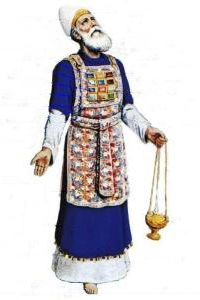
\includegraphics[width=50mm,scale=1.5]{Extras/Melchisedec.jpg}
\vspace{0.4in}  % Create a title for the document and write it in bold font
\LARGE{\textbf{\date}} % Again, do a line break
\linebreak 
% Create a subtitle \large{with Outlines, Statistics, Cross References, and Notes}
\vspace{0.5in}
\begin{flushleft}
\LARGE{Day \#46: Tuesday, 15 February 2022 PLAIN \\}\vspace{0.25in}
\LARGE{Numbers 16-18 Psalm 46 Proverb 15}
\end{flushleft}
\vspace{0.6in}
\bigskip

\normalsize{Xenia, Oh.\\}
\normalsize{created: \today}
\vspace{1.3in}

\end{flushright}
\end{titlepage}

\newpage 
\tableofcontents\hypertarget{TOC}{}

\hyphenation{A-bim-e-lech bre-thren E-phra-im  Gib-e-o-nites Jer-u-sa-lem through-out Phil-i-stines The-o-phil-us Am-a-le-kites ven-geance Mesh-el-e-mi-ah onan-ism Phar-a-oh thoughts grev-ous-ness Hach-a-liah adul-ter-er Shad-rach}

%%%%%%%%%%%%%%%%% EXTRA COLORS
%%%%%%%%%%%%%%%%% EXTRA COLORS
%%%%%%%%%%%%%%%%% EXTRA COLORS
\definecolor{champagne}{rgb}{0.97,0.91,0.81}
\definecolor{bone}{rgb}{0.89,0.85,0.79}

\definecolor{ForestGreen}{rgb}{0.00,0.29,0.098}
\definecolor{GIVING}{cmyk}{1,0.0,0.72,.1}

\definecolor{MLPE}{cmyk}{1,1,0,.45}
\definecolor{SOCCER}{cmyk}{.77, 0, .42, .49}
\definecolor{PAYBILL}{cmyk}{0,0.83,0.76,0.07}
\definecolor{SERMON}{cmyk}{.14,.9,0,.30} % aka seance \href{http://www.flatuicolorpicker.com/purple-cmyk-color-model/}{seance}
\definecolor{BIBLE}{cmyk}{0,.17,.74,.17}
\definecolor{WORKBLUE}{cmyk}{1, .5, 0, .6}
\definecolor{myOrange}{cmyk}{0, .4, .98, .03}
\definecolor{myTan}{cmyk}{0.0,.07,.17,.10}
\definecolor{myRed}{cmyk}{0,1,1,0}
\definecolor{myWhite}{cmyk}{0,0,0,0}
\definecolor{BLUESoD}{cmyk}{.97,.84,0,.04}
\definecolor{WHITE}{cmyk}{0,0,0,0}
\definecolor{OLDGOLD}{cmyk}{0.05,0.3,1.00,0}
\definecolor{CASTLETON}{cmyk}{1,0,0.31,0.66}
\definecolor{cadmiumgreen}{rgb}{0.0, 0.42, 0.24}
\definecolor{jungle}{rgb}{0.203,0.4882,0.1718}
\definecolor{MYGOLD}{rgb}{1,.84,0}

\definecolor{MYLIGHTGRAY}{rgb}{.85,.85,.85}

\definecolor{codegreen}{rgb}{0,0.6,0}
\definecolor{codegray}{rgb}{0.5,0.5,0.5}
\definecolor{codepurple}{rgb}{0.58,0,0.82}
\definecolor{backcolour}{rgb}{0.95,0.95,0.92}


\mdfdefinestyle{MyFrame}{%
    linecolor=blue,
    outerlinewidth=2pt,
    roundcorner=5pt,
    innertopmargin=\baselineskip,
    innerbottommargin=\baselineskip,
    innerrightmargin=10pt,
    innerleftmargin=10pt,
    backgroundcolor=gray!25!white}


\mdfdefinestyle{MyFrame2}{%
    linecolor=black,
    outerlinewidth=2pt,
    roundcorner=5pt,
    innertopmargin=\baselineskip,
    innerbottommargin=\baselineskip,
    innerrightmargin=10pt,
    innerleftmargin=10pt,
    backgroundcolor=yellow!25!white}


%%%%%
%% for PFTTIS list
%%%%%

%%% And Joseph said unto
\index[PFTTIS]{And Joseph said unto!Genesis!Gen 40:008}
\index[PFTTIS]{And Joseph said unto!Genesis!Gen 40:012}
\index[PFTTIS]{And Joseph said unto!Genesis!Gen 41:025}
\index[PFTTIS]{And Joseph said unto!Genesis!Gen 42:014}
\index[PFTTIS]{And Joseph said unto!Genesis!Gen 42:018}
\index[PFTTIS]{And Joseph said unto!Genesis!Gen 44:015}
\index[PFTTIS]{And Joseph said unto!Genesis!Gen 45:003}
\index[PFTTIS]{And Joseph said unto!Genesis!Gen 45:004}
\index[PFTTIS]{And Joseph said unto!Genesis!Gen 46:031}
\index[PFTTIS]{And Joseph said unto!Genesis!Gen 48:009}
\index[PFTTIS]{And Joseph said unto!Genesis!Gen 48:018}
\index[PFTTIS]{And Joseph said unto!Genesis!Gen 50:019}
\index[PFTTIS]{And Joseph said unto!Genesis!Gen 50:024}


%%% a shadow
\index[PFTTIS]{a shadow!1Chronicles!1Chr 029:15}
\index[PFTTIS]{a shadow!Job!Job 008:09}
\index[PFTTIS]{a shadow!Job!Job 014:02}
\index[PFTTIS]{a shadow!Job!Job 017:07}
\index[PFTTIS]{a shadow!Psalm!Psa 102:011}
\index[PFTTIS]{a shadow!Psalm!Psa 144:004}
\index[PFTTIS]{a shadow!Ecclesiastes!Eccl 006:012}
\index[PFTTIS]{a shadow!Ecclesiastes!Eccl 008:013}
\index[PFTTIS]{a shadow!Isaiah!Isa 04:006}
\index[PFTTIS]{a shadow!Isaiah!Isa 25:004}
\index[PFTTIS]{a shadow!Jonah!Jnh 04:06}
\index[PFTTIS]{a shadow!Colossians!Col 02:017}
\index[PFTTIS]{a shadow!Hebews!Heb 10:001}

%%% blessed is the man
\index[PFTTIS]{blessed is the man!Psalm!Psa 001:001}
\index[PFTTIS]{blessed is the man!Psalm!Psa 032:002}
\index[PFTTIS]{blessed is the man!Psalm!Psa 034:008}
\index[PFTTIS]{blessed is the man!Psalm!Psa 065:004}
\index[PFTTIS]{blessed is the man!Psalm!Psa 084:005}
\index[PFTTIS]{blessed is the man!Psalm!Psa 084:012}
\index[PFTTIS]{blessed is the man!Psalm!Psa 094:012}
\index[PFTTIS]{blessed is the man!Psalm!Psa 112:001}
\index[PFTTIS]{blessed is the man!Proverbs!Pro 008:034}
\index[PFTTIS]{blessed is the man!Isaiah!Isa 056:002}
\index[PFTTIS]{blessed is the man!Jeremiah!Jer 017:007}
\index[PFTTIS]{blessed is the man!Romans!Rom 004:008}
\index[PFTTIS]{blessed is the man!James!Jam 001:012}


%%% carry them
\index[PFTTIS]{carry them!Leviticus!Lev 14:045}
\index[PFTTIS]{carry them!Numbers!Num 11:012}
\index[PFTTIS]{carry them!Joshua!Jsh 04:003}
\index[PFTTIS]{carry them!1Samuel!1Sam 20:040}
\index[PFTTIS]{carry them!1Kings!1Kng 08:046}
\index[PFTTIS]{carry them!2Chronicles!2Chr 06:036}
\index[PFTTIS]{carry them!Ezra!Ezra 05:015}
\index[PFTTIS]{carry them!Isaiah!Isa 40:011}
\index[PFTTIS]{carry them!Isaiah!Isa 41:016}
\index[PFTTIS]{carry them!Isaiah!Isa 57:013}
\index[PFTTIS]{carry them!Jeremiah!Jer 20:004}
\index[PFTTIS]{carry them!Jeremiah!Jer 20:005}
\index[PFTTIS]{carry them!Jeremiah!Jer 43:012}


\index[PFTTIS]{good tidings!2Samuel!2Sam 18:027}
\index[PFTTIS]{good tidings!1Kings!1Ki 01:042}
\index[PFTTIS]{good tidings!2Kings!2Ki 07:009 (2x)}
\index[PFTTIS]{good tidings!Isaiah!Isa 40:009 (2x)}
\index[PFTTIS]{good tidings!Isaiah!Isa 41:007}
\index[PFTTIS]{good tidings!Isaiah!Isa 52:007}
\index[PFTTIS]{good tidings!Isaiah!Isa 61:001}
\index[PFTTIS]{good tidings!Nahum!Nah 01:005}
\index[PFTTIS]{good tidings!Luke!Lk 02:010}
\index[PFTTIS]{good tidings!1Thessalonians!1Thess 03:006}


%%% dead body
\index[PFTTIS]{dead body!Leviticus!Lev 21:011}
\index[PFTTIS]{dead body!Numbers!Num 06:006}
\index[PFTTIS]{dead body!Numbers!Num 09:006}
\index[PFTTIS]{dead body!Numbers!Num 09:007}
\index[PFTTIS]{dead body!Numbers!Num 09:010}
\index[PFTTIS]{dead body!Numbers!Num 09:011}
\index[PFTTIS]{dead body!Numbers!Num 09:013}
\index[PFTTIS]{dead body!Numbers!Num 09:016}
\index[PFTTIS]{dead body!2Kings!2Ki 08:005}
\index[PFTTIS]{dead body!Isaiah!Isa 26:019}
\index[PFTTIS]{dead body!Jeremiah!Jer 26:023}
\index[PFTTIS]{dead body!Jeremiah!Jer 36:030}
\index[PFTTIS]{dead body!Haggai!Hag 02:013}

%%% great sea
\index[PFTTIS]{great sea!Numbers!Num 34:006}
\index[PFTTIS]{great sea!Numbers!Num 34:007}
\index[PFTTIS]{great sea!Joshua!Jos 01:004}
\index[PFTTIS]{great sea!Joshua!Jos 09:001}
\index[PFTTIS]{great sea!Joshua!Jos 15:012}
\index[PFTTIS]{great sea!Joshua!Jos 15:047}
\index[PFTTIS]{great sea!Joshua!Jos 23:004}
\index[PFTTIS]{great sea!Ezekiel!Eze 47:010}
\index[PFTTIS]{great sea!Ezekiel!Eze 47:015}
\index[PFTTIS]{great sea!Ezekiel!Eze 47:019}
\index[PFTTIS]{great sea!Ezekiel!Eze 47:020}
\index[PFTTIS]{great sea!Ezekiel!Eze 48:028}
\index[PFTTIS]{great sea!Daniel!Dan 07:002}


%%% have forsaken me
\index[PFTTIS]{have forsaken me!Judges!Jdg 10:013}
\index[PFTTIS]{have forsaken me!1Samuel!1Sam 08:008}
\index[PFTTIS]{have forsaken me!1Kings!1Ki 11:033}
\index[PFTTIS]{have forsaken me!2Kings!2Ki 22:017}
\index[PFTTIS]{have forsaken me!2Chronicles!2Chr 12:005}
\index[PFTTIS]{have forsaken me!2Chronicles!2Chr 34:025}
\index[PFTTIS]{have forsaken me!Jeremiah!Jer 01:016}
\index[PFTTIS]{have forsaken me!Jeremiah!Jer 02:013}
\index[PFTTIS]{have forsaken me!Jeremiah!Jer 05:007}
\index[PFTTIS]{have forsaken me!Jeremiah!Jer 05:019}
\index[PFTTIS]{have forsaken me!Jeremiah!Jer 16:011 (2x)}
\index[PFTTIS]{have forsaken me!Jeremiah!Jer 19:004}

%%% no king
\index[PFTTIS]{no king!Judges!Jdg 17:06}
\index[PFTTIS]{no king!Judges!Jdg 18:01}
\index[PFTTIS]{no king!Judges!Jdg 19:01}
\index[PFTTIS]{no king!Judges!Jdg 21:25}
\index[PFTTIS]{no king!1Kings!1Ki 22:47}
\index[PFTTIS]{no king!2Kings!2Ki 23:25}
\index[PFTTIS]{no king!Nehemiah!Neh 13:26}
\index[PFTTIS]{no king!Psalms!Psa 033:016}
\index[PFTTIS]{no king!Proverbs!Pro 30:27}
\index[PFTTIS]{no king!Daniel!Dan 02:10}
\index[PFTTIS]{no king!Hosea!Hos 10:03}
\index[PFTTIS]{no king!Micah!Mic 04:09}
\index[PFTTIS]{no king!John!Jhn 19:15}


%%% rebellious house
\index[PFTTIS]{rebellious house!Exodus!Exo 02:005}
\index[PFTTIS]{rebellious house!Exodus!Exo 02:006}
\index[PFTTIS]{rebellious house!Exodus!Exo 02:008}
\index[PFTTIS]{rebellious house!Exodus!Exo 03:009}
\index[PFTTIS]{rebellious house!Exodus!Exo 03:026}
\index[PFTTIS]{rebellious house!Exodus!Exo 03:027}
\index[PFTTIS]{rebellious house!Exodus!Exo 12:002 (2x)}
\index[PFTTIS]{rebellious house!Exodus!Exo 12:003}
\index[PFTTIS]{rebellious house!Exodus!Exo 12:009}
\index[PFTTIS]{rebellious house!Exodus!Exo 12:025}
\index[PFTTIS]{rebellious house!Exodus!Exo 17:012}
\index[PFTTIS]{rebellious house!Exodus!Exo 24:003}

%%% seek him
\index[PFTTIS]{seek him!Deuteronomy!Deu 04:029}\index[PFTTIS]{seek him!1Samuel!1Sam 23:025}
\index[PFTTIS]{seek him!1Chronicles!1Chr 28:009}
\index[PFTTIS]{seek him!2Chronicles!1Chr 15:002}
\index[PFTTIS]{seek him!Ezra!Ezr 08:022}
\index[PFTTIS]{seek him!Psalms!Psa 022:026}
\index[PFTTIS]{seek him!Psalms!Psa 024:006}
\index[PFTTIS]{seek him!Psalms!Psa 119:002}
\index[PFTTIS]{seek him!SoS!SoS 03:002}
\index[PFTTIS]{seek him!SoS!SoS 06:001}
\index[PFTTIS]{seek him!Hosea!Hos 07:010}
\index[PFTTIS]{seek him!Amos!Amo 05:008}
\index[PFTTIS]{seek him!Hebrews!Heb 11:0063}


%%% seek ye
\index[PFTTIS]{seek ye!Isaiah!Isa 34:016}
\index[PFTTIS]{seek ye!Isaiah!Isa 45:019}
\index[PFTTIS]{seek ye!Isaiah!Isa 55:006}
\index[PFTTIS]{seek ye!Amos!Amos 5:004}
\index[PFTTIS]{seek ye!John!John 1:38}
\index[PFTTIS]{seek ye!John!John 18:4}
\index[PFTTIS]{seek ye!John!John 18:7}
\index[PFTTIS]{seek ye!Matthew!Matt 6:33}
\index[PFTTIS]{seek ye!Numbers!Num 16:10}
\index[PFTTIS]{seek ye!Luke!Luke 12:31}
\index[PFTTIS]{seek ye!Luke!Luke 24:5}
\index[PFTTIS]{seek ye!Psalm!Psa 27:8}
\index[PFTTIS]{seek ye!Zephaniah!Zeph 2:3}

%%% the uncircumcised
\index[PFTTIS]{the uncircumcised!Genesis!Gen 17:014}
\index[PFTTIS]{the uncircumcised!Judges!Jdg 14:003}
\index[PFTTIS]{the uncircumcised!Judges!Jdg 15:018}
\index[PFTTIS]{the uncircumcised!2Samuel!2Sam 01:020}
\index[PFTTIS]{the uncircumcised!Isaiah!Isa 02:001}
\index[PFTTIS]{the uncircumcised!Jeremiah!Jer 09:025}
\index[PFTTIS]{the uncircumcised!Ezekiel!Eze 28:010}
\index[PFTTIS]{the uncircumcised!Ezekiel!Eze 31:018}
\index[PFTTIS]{the uncircumcised!Ezekiel!Eze 32:019}
\index[PFTTIS]{the uncircumcised!Ezekiel!Eze 32:027}
\index[PFTTIS]{the uncircumcised!Ezekiel!Eze 32:028}
\index[PFTTIS]{the uncircumcised!Ezekiel!Eze 32:029}
\index[PFTTIS]{the uncircumcised!Ezekiel!Eze 32:032}

%%% worship him
\index[PFTTIS]{worship him!Psalms!Psa 97:007}
\index[PFTTIS]{worship him!Zephaniah!Zeph 02:011}
\index[PFTTIS]{worship him!Matthew!Matt 02:002}
\index[PFTTIS]{worship him!Matthew!Matt 02:008}
\index[PFTTIS]{worship him!John!John 04:023}
\index[PFTTIS]{worship him!John!John 04:024 (2x)} 
\index[PFTTIS]{worship him!Acts!Acts 17:023}
\index[PFTTIS]{worship him!Hebrews!Heb 01:006}
\index[PFTTIS]{worship him!Revelation!Rev 04:010}
\index[PFTTIS]{worship him!Revelation!Rev 13:008}
\index[PFTTIS]{worship him!Revelation!Rev 14:007}
\index[PFTTIS]{worship him!Revelation!Rev 19:010}


%%%%%
%% for PFTTIS list
%%%%%

%%% afflictions
\index[WFTTIS]{afflictions!Psalms!Psa 34:019}
\index[WFTTIS]{afflictions!Psalms!Psa 132:001}
\index[WFTTIS]{afflictions!Acts!Acts 07:010}
\index[WFTTIS]{afflictions!Acts!Acts 20:023}
\index[WFTTIS]{afflictions!2Corinthians!2Cor 06:004}
\index[WFTTIS]{afflictions!Colossians!Col 01:024}
\index[WFTTIS]{afflictions!1Thessalonians!1Thess 03:003}
\index[WFTTIS]{afflictions!2Timothy!2Tim 01:008}
\index[WFTTIS]{afflictions!2Timothy!2Tim 03:011}
\index[WFTTIS]{afflictions!2Timothy!2Tim 04:005}
\index[WFTTIS]{afflictions!Hebrews!Heb 10:032}
\index[WFTTIS]{afflictions!Hebrews!Heb 10:033}
\index[WFTTIS]{afflictions!1Peter!1Pet 05:009}

%%% acsend
\index[WFTTIS]{acsend!Joshua!Jos 06:05}
\index[WFTTIS]{acsend!Psalm!Psa 024:003}
\index[WFTTIS]{acsend!Psalm!Psa 135:007}
\index[WFTTIS]{acsend!Psalm!Psa 139:008}
\index[WFTTIS]{acsend!Isaiah!Isa 14:013}
\index[WFTTIS]{acsend!Isaiah!Isa 14:014}
\index[WFTTIS]{acsend!Jeremiah!Jer 10:013}
\index[WFTTIS]{acsend!Jeremiah!Jer 51:016}
\index[WFTTIS]{acsend!Ezekiel!Eze 38:009}
\index[WFTTIS]{acsend!John!John 06:062}
\index[WFTTIS]{acsend!John!John 20:017}
\index[WFTTIS]{acsend!Romans!Rom 10:006}
\index[WFTTIS]{acsend!Revelation!Rev 17:008}

%%% Assyrian
\index[WFTTIS]{Assyrian!Isaiah!Isa 10:005}
\index[WFTTIS]{Assyrian!Isaiah!Isa 10:024}
\index[WFTTIS]{Assyrian!Isaiah!Isa 14:025}
\index[WFTTIS]{Assyrian!Isaiah!Isa 19:023}
\index[WFTTIS]{Assyrian!Isaiah!Isa 23:013}
\index[WFTTIS]{Assyrian!Isaiah!Isa 30:031}
\index[WFTTIS]{Assyrian!Isaiah!Isa 31:008}
\index[WFTTIS]{Assyrian!Isaiah!Isa 52:004}
\index[WFTTIS]{Assyrian!Ezekiel!Eze 31:003}
\index[WFTTIS]{Assyrian!Hosea!Hos 05:013}
\index[WFTTIS]{Assyrian!Hosea!Hos 11:005}
\index[WFTTIS]{Assyrian!Micah!Hos 05:005}
\index[WFTTIS]{Assyrian!Micah!Hos 05:006}

%%% blot
\index[WFTTIS]{blot!Exodus!Exo 32:032}
\index[WFTTIS]{blot!Exodus!Exo 32:033}
\index[WFTTIS]{blot!Numbers!Num 05:026}
\index[WFTTIS]{blot!Deuteronomy!Deut 09:014}
\index[WFTTIS]{blot!Deuteronomy!Deut 25:019}
\index[WFTTIS]{blot!Deuteronomy!Deut 29:020}
\index[WFTTIS]{blot!2Kings!2Ki 14:027}
\index[WFTTIS]{blot!Job!Job 31:007}
\index[WFTTIS]{blot!Psalms!Psa 51:001}
\index[WFTTIS]{blot!Psalms!Psa 51:009}
\index[WFTTIS]{blot!Proverbs!Pro 09:007}
\index[WFTTIS]{blot!Jeremiah!Jer 18:023}
\index[WFTTIS]{blot!Revelation!Rev 03:005}


%%% chain
\index[WFTTIS]{chain!Genesis!Gen 41:042}
\index[WFTTIS]{chain!1Kings!1Ki 07:017}
\index[WFTTIS]{chain!Psalms!Psa 73:006}
\index[WFTTIS]{chain!SoS!Sos 04:009}
\index[WFTTIS]{chain!Lamentations!Lam 03:007}
\index[WFTTIS]{chain!Ezekiel!Eze 07:023}
\index[WFTTIS]{chain!Ezekiel!Eze 16:011}
\index[WFTTIS]{chain!Daniel!Dan 05:007}
\index[WFTTIS]{chain!Daniel!Dan 05:016}
\index[WFTTIS]{chain!Daniel!Dan 05:029}
\index[WFTTIS]{chain!Acts!Acts 28:020}
\index[WFTTIS]{chain!2Timothy!2Tim 01:016}
\index[WFTTIS]{chain!Revelation!Rev 20:001}


%%% controversy
\index[WFTTIS]{controversy!Deuteronomy!Deu 17:008}
\index[WFTTIS]{controversy!Deuteronomy!Deu 19:017}
\index[WFTTIS]{controversy!Deuteronomy!Deu 21:005}
\index[WFTTIS]{controversy!Deuteronomy!Deu 25:001}
\index[WFTTIS]{controversy!2Samuel!2Sam 15:002}
\index[WFTTIS]{controversy!Isaiah!Isa 34:008}
\index[WFTTIS]{controversy!Jeremiah!Jer 25:031}
\index[WFTTIS]{controversy!Ezekiel!Eze 44:024}
\index[WFTTIS]{controversy!Hosea!Hos 04:001}
\index[WFTTIS]{controversy!Hosea!Hos 12:002}
\index[WFTTIS]{controversy!Micah!Mic 06:002 (2x)}
\index[WFTTIS]{controversy!1Timothy!1Tim 03:016}


%%% Dagon/Dagon's
\index[WFTTIS]{Dagon!Judges!Jdg 16:023}
\index[WFTTIS]{Dagon!1Samuel!1Sam 05:002 (2x)}
\index[WFTTIS]{Dagon!1Samuel!1Sam 05:003 (2x)}
\index[WFTTIS]{Dagon!1Samuel!1Sam 05:004 (3x)}
\index[WFTTIS]{Dagon!1Samuel!1Sam 05:005 (3x)}
\index[WFTTIS]{Dagon!1Samuel!1Sam 05:007}
\index[WFTTIS]{Dagon!1Chronicles!1Chr 10:010}

%%% disobedient
\index[WFTTIS]{disobedient!1Kings!1Ki 13:026}
\index[WFTTIS]{disobedient!Nehemiah!Neh 09:026}
\index[WFTTIS]{disobedient!Luke!Luke 01:017}
\index[WFTTIS]{disobedient!Acts!Acts 26:019}
\index[WFTTIS]{disobedient!Romans!Rom 01:030}
\index[WFTTIS]{disobedient!Romans!Rom 10:021}
\index[WFTTIS]{disobedient!1Timothy!1Tim 01:009}
\index[WFTTIS]{disobedient!2Timothy!2Tim 03:002}
\index[WFTTIS]{disobedient!Titus!Titus 01:016}
\index[WFTTIS]{disobedient!Titus!Titus 03:003}
\index[WFTTIS]{disobedient!1Peter!1Pet 02:007}
\index[WFTTIS]{disobedient!1Peter!1Pet 02:008}
\index[WFTTIS]{disobedient!1Peter!1Pet 03:020}


%%% doubt
\index[WFTTIS]{doubt!Genesis!Gen 37:033}
\index[WFTTIS]{doubt!Deuteronomy!Deu 28:066}
\index[WFTTIS]{doubt!Job!Job 12:002}
\index[WFTTIS]{doubt!Matthew!Matt 14:031}
\index[WFTTIS]{doubt!Matthew!Matt 21:021}
\index[WFTTIS]{doubt!Mark!Mk 11:023}
\index[WFTTIS]{doubt!Luke!Lk 11:020}
\index[WFTTIS]{doubt!John!Jhn 10:024}
\index[WFTTIS]{doubt!Acts!Acts 02:012}
\index[WFTTIS]{doubt!Acts!Acts 28:004}
\index[WFTTIS]{doubt!1Corinthians!1Cor 09:010}
\index[WFTTIS]{doubt!Galatians!Gal 04:020}
\index[WFTTIS]{doubt!1John!1Jhn 02:019}


%%% dungeon
\index[WFTTIS]{dungeon!Genesis!Gen 40:015}
\index[WFTTIS]{dungeon!Genesis!Gen 41:014}
\index[WFTTIS]{dungeon!Exodus!Exo 12:029}
\index[WFTTIS]{dungeon!Jeremiah!Jer 37:016}
\index[WFTTIS]{dungeon!Jeremiah!Jer 38:006 (2x)}
\index[WFTTIS]{dungeon!Jeremiah!Jer 38:007}
\index[WFTTIS]{dungeon!Jeremiah!Jer 38:009}
\index[WFTTIS]{dungeon!Jeremiah!Jer 38:010}
\index[WFTTIS]{dungeon!Jeremiah!Jer 38:011}
\index[WFTTIS]{dungeon!Jeremiah!Jer 38:013}
\index[WFTTIS]{dungeon!Lamentations!Lam 03:053}
\index[WFTTIS]{dungeon!Lamentations!Lam 03:055}


%%% error
\index[WFTTIS]{error!2Samuel!2Sam 06:007}
\index[WFTTIS]{error!Job!Job 19:004}
\index[WFTTIS]{error!Ecclesiastes!Ecc 05:006}
\index[WFTTIS]{error!Ecclesiastes!Ecc 10:005}
\index[WFTTIS]{error!Isaiah!Isa 32:006}
\index[WFTTIS]{error!Daniel!Dan 06:004}
\index[WFTTIS]{error!Matthew!Matt 27:064}
\index[WFTTIS]{error!Romans!Rom 01:027}
\index[WFTTIS]{error!James!Jam 05:020}
\index[WFTTIS]{error!2Peter!2Pet 02:018}
\index[WFTTIS]{error!2Peter!2Pet 03:017}
\index[WFTTIS]{error!1John!1Jn 04:006}
\index[WFTTIS]{error!Jude!Jude 01:011}

%%% fourish
\index[WFTTIS]{fourish!Psalms!Psa 072:007}
\index[WFTTIS]{fourish!Psalms!Psa 072:016}
\index[WFTTIS]{fourish!Psalms!Psa 092:007}
\index[WFTTIS]{fourish!Psalms!Psa 092:012}
\index[WFTTIS]{fourish!Psalms!Psa 092:013}
\index[WFTTIS]{fourish!Psalms!Psa 132:018}
\index[WFTTIS]{fourish!Proverbs!Pro 11:28}
\index[WFTTIS]{fourish!Proverbs!Pro 14:11}
\index[WFTTIS]{fourish!Ecclesiastes!Ecc 12:05}
\index[WFTTIS]{fourish!SongOfSolomon!SOS 07:12}
\index[WFTTIS]{fourish!Isaiah!Isa 17:11}
\index[WFTTIS]{fourish!Isaiah!Isa 66:14}
\index[WFTTIS]{fourish!Ezekiel!Eze 17:24}




%%% giants
\index[WFTTIS]{giants!Genesis!Gen 06:004}
\index[WFTTIS]{giants!Numbers!Num 13:033}
\index[WFTTIS]{giants!Deuteronomy!Deut 02:011}
\index[WFTTIS]{giants!Deuteronomy!Deut 02:021}
\index[WFTTIS]{giants!Deuteronomy!Deut 03:011}
\index[WFTTIS]{giants!Deuteronomy!Deut 03:013}
\index[WFTTIS]{giants!Joshua!Josh 12:004}
\index[WFTTIS]{giants!Joshua!Josh 13:012}
\index[WFTTIS]{giants!Joshua!Josh 15:008}
\index[WFTTIS]{giants!Joshua!Josh 17:015}
\index[WFTTIS]{giants!Joshua!Josh 16:016}

%%% good man
\index[WFTTIS]{good man!2 Samuel!2Sa 18:27}
%(1) Psalms 37:23 [5]
%(1) Psalms 112:5 [2]
%(1) Proverbs 12:2 [2]
%(1) Proverbs 13:22 [2]
%(1) Proverbs 14:14 [14]
%(1) Micah 7:2 [2]
%(1) Matthew 12:35 [2]
%(1) Luke 6:45 [2]
%(1) Luke 23:50 [15]
%(1) John 7:12 [17]
%(1) Acts 11:24 [5]
%(1) Romans 5:7 [14]

%%% Hinnom
\index[WFTTIS]{Hinnom!Joshua!Jsh 15:008}
\index[WFTTIS]{Hinnom!Joshua!Jsh 18:016}
\index[WFTTIS]{Hinnom!2Kings!2Ki 23:010}
\index[WFTTIS]{Hinnom!2Chronicles!2Chr 28:003}
\index[WFTTIS]{Hinnom!2Chronicles!2Chr 33:006}
\index[WFTTIS]{Hinnom!Nehemiah!Neh 11:030}
\index[WFTTIS]{Hinnom!Jeremiah!Jer 07:031}
\index[WFTTIS]{Hinnom!Jeremiah!Jer 07:032}
\index[WFTTIS]{Hinnom!Jeremiah!Jer 19:002}
\index[WFTTIS]{Hinnom!Jeremiah!Jer 19:006}
\index[WFTTIS]{Hinnom!Jeremiah!Jer 32:035}

%%% inclined
\index[WFTTIS]{inclined!Judges!Jdg 09:003}
\index[WFTTIS]{inclined!Psalms!Psa 040:001}
\index[WFTTIS]{inclined!Psalms!Psa 116:002}
\index[WFTTIS]{inclined!Psalms!Psa 119:112}
\index[WFTTIS]{inclined!Proverbs!Pro 05:13}
\index[WFTTIS]{inclined!Jeremiah!Jer 07:24}
\index[WFTTIS]{inclined!Jeremiah!Jer 07:26}
\index[WFTTIS]{inclined!Jeremiah!Jer 11:08}
\index[WFTTIS]{inclined!Jeremiah!Jer 17:23}
\index[WFTTIS]{inclined!Jeremiah!Jer 25:04}
\index[WFTTIS]{inclined!Jeremiah!Jer 34:14}
\index[WFTTIS]{inclined!Jeremiah!Jer 35:15}
\index[WFTTIS]{inclined!Jeremiah!Jer 44:05}


%%% laughed
\index[WFTTIS]{laughed!Genesis!Gen 17:017}
\index[WFTTIS]{laughed!Genesis!Gen 18:012}
\index[WFTTIS]{laughed!Genesis!Gen 18:015}
\index[WFTTIS]{laughed!2Kings!2Ki 19:021}
\index[WFTTIS]{laughed!2Chronicles!2Chr 30:010}
\index[WFTTIS]{laughed!Nehemiah!Neh 02:019}
\index[WFTTIS]{laughed!Job!Job 12:004}
\index[WFTTIS]{laughed!Job!Job 29:024}
\index[WFTTIS]{laughed!Isaiah!Isa 37:022}
\index[WFTTIS]{laughed!Ezekiel!Ezek 23:032}
\index[WFTTIS]{laughed!Matthew!Matt 09:024}
\index[WFTTIS]{laughed!Mark!Mk 05:040}
\index[WFTTIS]{laughed!Luke!Lk 08:053}

%%% liar
\index[WFTTIS]{liar!Job!Job 24:025}
\index[WFTTIS]{liar!Proverbs!Pro 17:004}
\index[WFTTIS]{liar!Proverbs!Pro 19:022}
\index[WFTTIS]{liar!Proverbs!Pro 30:006}
\index[WFTTIS]{liar!Jeremiah!Jer 15:018}
\index[WFTTIS]{liar!John!Jhn 08:044}
\index[WFTTIS]{liar!John!Jhn 08:055}
\index[WFTTIS]{liar!Romans!Rom 03:004}
\index[WFTTIS]{liar!1John!1Jhn 01:010}
\index[WFTTIS]{liar!1John!1Jhn 02:004}
\index[WFTTIS]{liar!1John!1Jhn 02:022}
\index[WFTTIS]{liar!1John!1Jhn 04:020}
\index[WFTTIS]{liar!1John!1Jhn 05:010}

%%% palsy
\index[WFTTIS]{palsy!Matthew!Matt 04:024}
\index[WFTTIS]{palsy!Matthew!Matt 08:006}
\index[WFTTIS]{palsy!Matthew!Matt 09:002}
\index[WFTTIS]{palsy!Matthew!Matt 09:006}
\index[WFTTIS]{palsy!Mark!Mk 02:003}
\index[WFTTIS]{palsy!Mark!Mk 02:004}
\index[WFTTIS]{palsy!Mark!Mk 02:005}
\index[WFTTIS]{palsy!Mark!Mk 02:009}
\index[WFTTIS]{palsy!Mark!Mk 02:010}
\index[WFTTIS]{palsy!Luke!Lk 05:018}
\index[WFTTIS]{palsy!Luke!Lk 05:024}
\index[WFTTIS]{palsy!Acts!Acts 09:033}

%%% Profitable
\index[WFTTIS]{profitable!Job!Job 22:002 (2x)}
\index[WFTTIS]{profitable!Ecclesiastes!Ecc 10:010}
\index[WFTTIS]{profitable!Isaiah!Isa 44:010}
\index[WFTTIS]{profitable!Jeremiah!Jer 13:007}
\index[WFTTIS]{profitable!Matthew!Matt 05:029}
\index[WFTTIS]{profitable!Matthew!Matt 05:030}
\index[WFTTIS]{profitable!Acts!Acts 20:020}
\index[WFTTIS]{profitable!1Timothy!1Tim 04:008}
\index[WFTTIS]{profitable!2Timothy!2Tim 03:016}
\index[WFTTIS]{profitable!2Timothy!2Tim 04:011}
\index[WFTTIS]{profitable!Titus!Titus 03:008}
\index[WFTTIS]{profitable!Philemon!Phlm 01:011}

%%% Rechab
\index[WFTTIS]{Rechab!2Samuel!2Sam 04:002}
\index[WFTTIS]{Rechab!2Samuel!2Sam 04:005}
\index[WFTTIS]{Rechab!2Samuel!2Sam 04:006}
\index[WFTTIS]{Rechab!2Samuel!2Sam 04:009}
\index[WFTTIS]{Rechab!2KIngs!2Ki 10:015}
\index[WFTTIS]{Rechab!2KIngs!2Ki 10:023}
\index[WFTTIS]{Rechab!1Chronicles!1Chr 02:055}
\index[WFTTIS]{Rechab!Nehemiah!Neh 03:014}
\index[WFTTIS]{Rechab!Jeremiah!Jer 35:006}
\index[WFTTIS]{Rechab!Jeremiah!Jer 35:008}
\index[WFTTIS]{Rechab!Jeremiah!Jer 35:014}
\index[WFTTIS]{Rechab!Jeremiah!Jer 35:016}
\index[WFTTIS]{Rechab!Jeremiah!Jer 35:019}

%%% serpents
\index[WFTTIS]{serpents!Exodus!Exo 07:012}
\index[WFTTIS]{serpents!Numbers!Num 21:006}
\index[WFTTIS]{serpents!Numbers!Num 21:007}
\index[WFTTIS]{serpents!Deuteronomy!Deu 08:015}
\index[WFTTIS]{serpents!Deuteronomy!Deu 32:024}
\index[WFTTIS]{serpents!Jeremiah!Jer 08:017}
\index[WFTTIS]{serpents!Matthew!Matt 10:016}
\index[WFTTIS]{serpents!Matthew!Matt 23:033}
\index[WFTTIS]{serpents!Mark!Mk 16:018}
\index[WFTTIS]{serpents!Luke!Lk 10:019}
\index[WFTTIS]{serpents!1Corinthians!1Cor 10:009}
\index[WFTTIS]{serpents!James!Jas 03:007}
\index[WFTTIS]{serpents!Revelation!Rev 09:019}

%%% short
\index[WFTTIS]{short!Numbers!Num 11:023}
\index[WFTTIS]{short!2Kings!2Ki 10:032}
\index[WFTTIS]{short!Job!Job 17:012}
\index[WFTTIS]{short!Job!Job 20:005}
\index[WFTTIS]{short!Psalms!Psa 89:047}
\index[WFTTIS]{short!Romans!Rom 03:023}
\index[WFTTIS]{short!Romans!Rom 09:028  (2x)}
\index[WFTTIS]{short!1Corinthians!1Cor 07:029}
\index[WFTTIS]{short!1Thessalonians!1Thess 02:017}
\index[WFTTIS]{short!Hebrews!Heb 04:001}
\index[WFTTIS]{short!Revelation!Rev 12:012}
\index[WFTTIS]{short!Revelation!Rev 17:010}

%%% smiteth
\index[WFTTIS]{smiteth!Exodus!Exo 21:012}
\index[WFTTIS]{smiteth!Exodus!Exo 21:15}
\index[WFTTIS]{smiteth!Deuteronomy!Dt 25:11}
\index[WFTTIS]{smiteth!Deuteronomy!Dt 27:24}
\index[WFTTIS]{smiteth!Joshua!Jsh 15:16}
\index[WFTTIS]{smiteth!Judges!Jdg 15:16}
\index[WFTTIS]{smiteth!2 Samuel!2Sa 05:08}
\index[WFTTIS]{smiteth!1Chronicles!1Chr 11:06}
\index[WFTTIS]{smiteth!Job!1Chr 26:12}
\index[WFTTIS]{smiteth!Isaiah!Isa 09:13}
\index[WFTTIS]{smiteth!Lamentations!Lam 03:30}
\index[WFTTIS]{smiteth!Ezekiel!Eze 07:09}
\index[WFTTIS]{smiteth!Luke!Lk 06:29}



%%% vanities
\index[WFTTIS]{vanities!Deuteronomy!Deut 21:021}
\index[WFTTIS]{vanities!1Kings!1Ki 16:013}
\index[WFTTIS]{vanities!1Kings!1Ki 16:026}
\index[WFTTIS]{vanities!Psalms!Psa 031:006}
\index[WFTTIS]{vanities!Ecclesiastes!Ecc 01:002 (2x)}
\index[WFTTIS]{vanities!Ecclesiastes!Ecc 05:007}
\index[WFTTIS]{vanities!Ecclesiastes!Ecc 12:008}
\index[WFTTIS]{vanities!Jeremiah!Jer 08:019}
\index[WFTTIS]{vanities!Jeremiah!Jer 10:008}
\index[WFTTIS]{vanities!Jeremiah!Jer 14:022}
\index[WFTTIS]{vanities!Jonah!Jnh 02:008}
\index[WFTTIS]{vanities!Acts!Acts 14:015}



%%%%%
%% for PFTTIS list
%%%%%

%%% worm
\index[WFITV]{worm!Exodus!Exo 16:024}
\index[WFITV]{worm!Job!Job 17:014}
\index[WFITV]{worm!Job!Job 24:029}
\index[WFITV]{worm!Job!Job 25:005 (2x)}
\index[WFITV]{worm!Psalms!Psa 022:006}
\index[WFITV]{worm!Isaiah!Isa 14:011}
\index[WFITV]{worm!Isaiah!Isa 41:014}
\index[WFITV]{worm!Isaiah!Isa 51:008}
\index[WFITV]{worm!Isaiah!Isa 66:024}
\index[WFITV]{worm!Jonah!Jnh 04:007}
\index[WFITV]{worm!Mark!Mk 09:044}
\index[WFITV]{worm!Mark!Mk 09:046}
\index[WFITV]{worm!Mark!Mk 09:048}


%\subsubsection{Title}
%\textbf{Introduction:} Isaiah 46 
%\index[speaker]{Speaker!Isaiah 49 (Title}
%\index[series]{Book (Speaker)!IPassage (Title)}
%\index[date]{2017/07/09!Isaiah 49 (Title)}
%\begin{compactenum}[I.]
%    \item  \textbf{Point} \index[scripture]{Isaiah!IPassage} (IPassage)
%\end{compactenum}




  


%\input{02OT-Exodus/ExodusIntroduction}
\newpage
\begin{figure}
\begin{center}
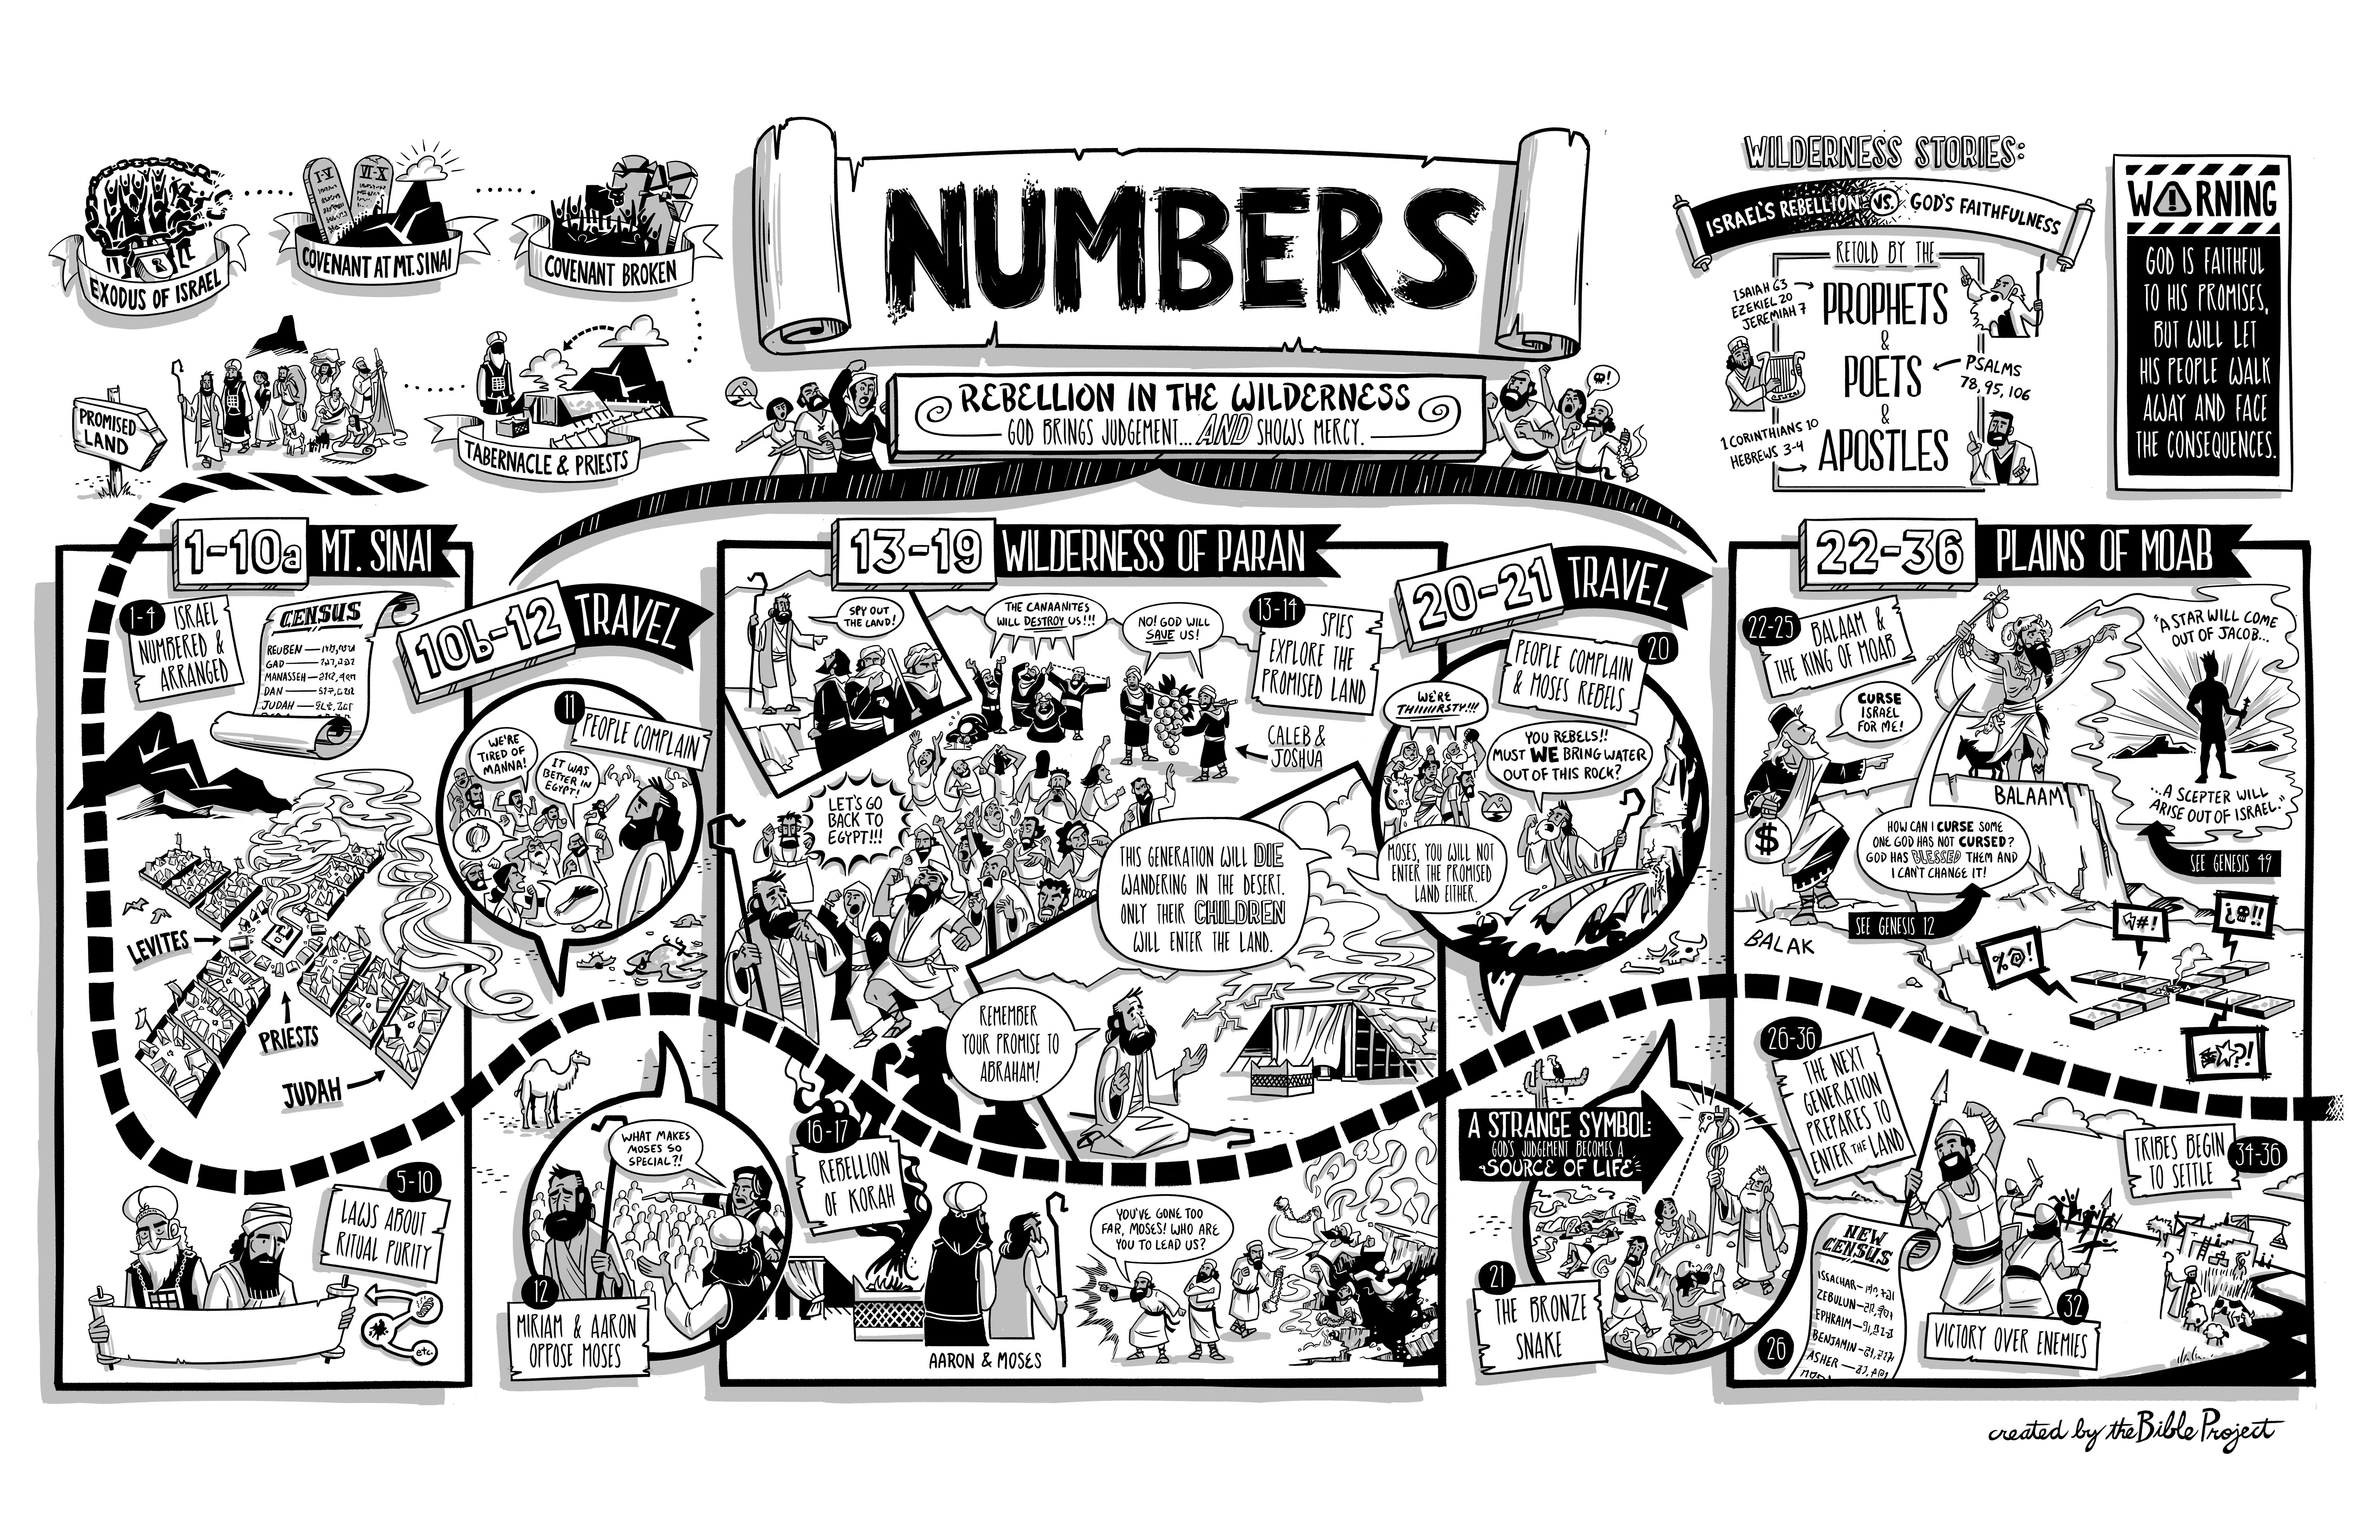
\includegraphics[scale=0.5, angle=90]{04OT-Numbers/References/BibleProject-Numbers.jpg}
\caption[Numbers from the Bible Project]{Numbers from the Bible Project}
\label{fig:Numbers from the Bible Project}
\end{center}
\end{figure}

\newpage
\begin{figure}
\begin{center}
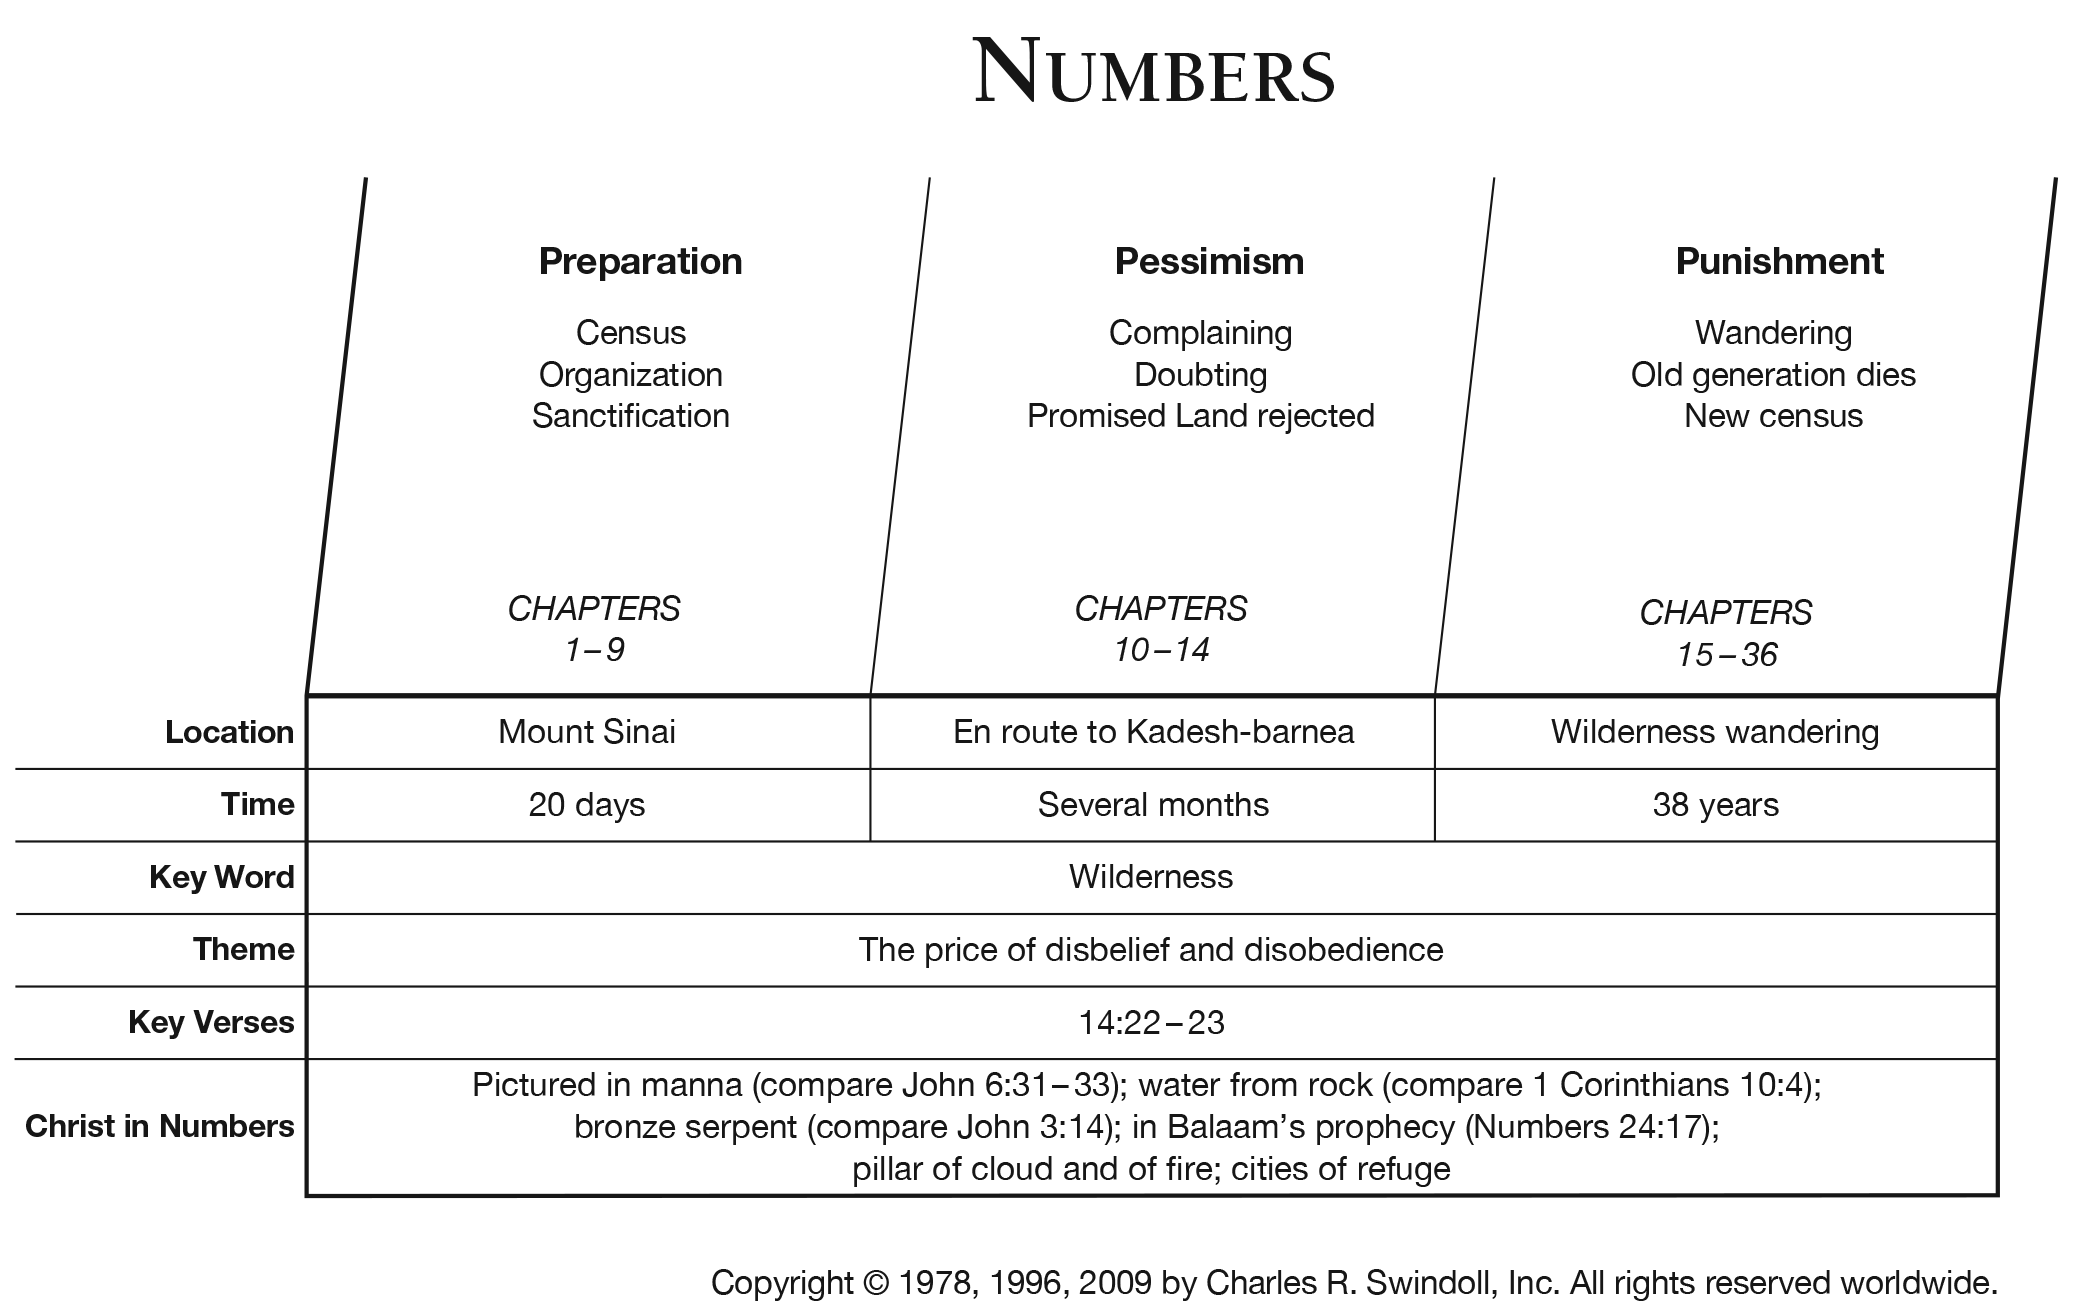
\includegraphics[scale=0.3, angle=90]{04OT-Numbers/References/Swindoll-Numbers.png}
\caption[Numbers by Swindoll]{Numbers by Swindoll}
\label{fig:Numbers by Swindoll}
\end{center}
\end{figure}

\newpage
\begin{figure}
\begin{center}
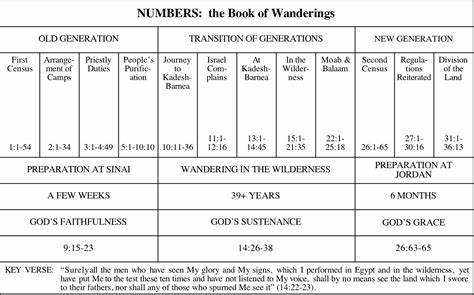
\includegraphics[scale=1.2, angle=90]{04OT-Numbers/References/Numbers.jpg}
\caption[Numbers by Unknown]{Numbers by Unknown}
\label{fig:Numbers by Unknown}
\end{center}
\end{figure}

\newpage
\begin{figure}
\begin{center}
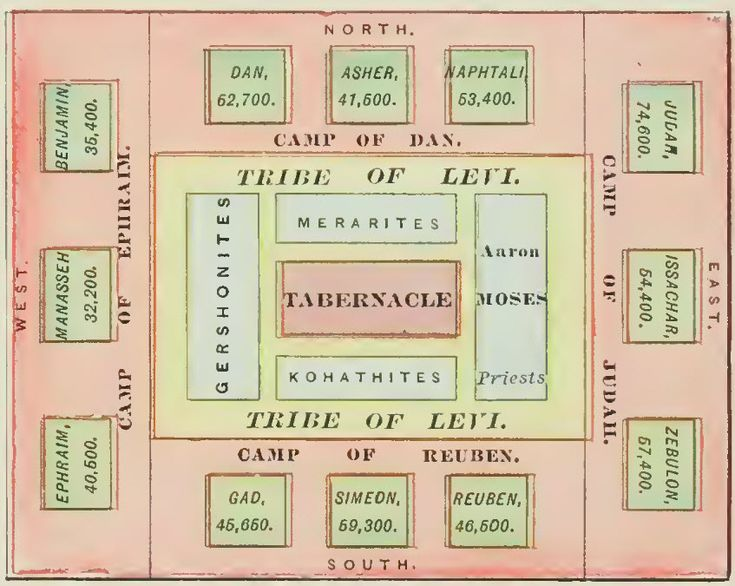
\includegraphics[scale=.8, angle=0]{04OT-Numbers/References/LayoutOfTribesAndTabernacle.jpg}
\caption[Layout of Tribes and Tabernacle]{Layout of Tribes and Tabernacle}
\label{fig:Layout of Tribes and Tabernacle}
\end{center}
\end{figure}


\chapter{Numbers 16}

\begin{figure}
  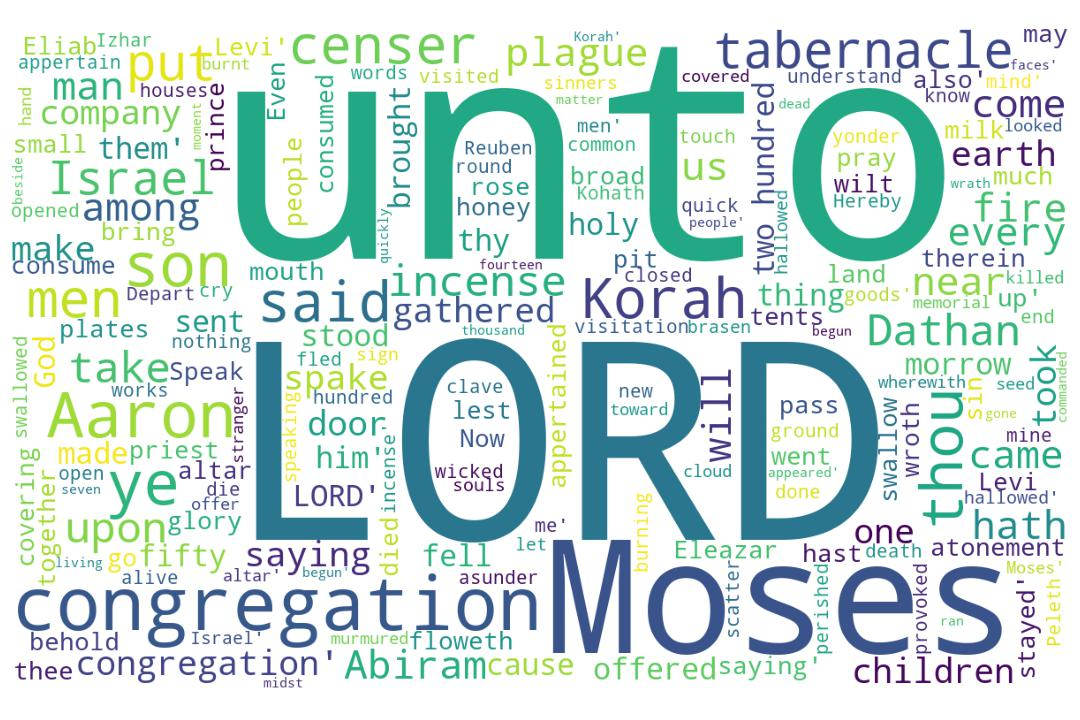
\includegraphics[width=\linewidth]{04OT-Numbers/Numbers16-WordCloud.jpg}
  \caption{Numbers 16 Word Cloud}
  \label{fig:Numbers 16 word Cloud}
\end{figure}

\marginpar{\scriptsize \centering \fcolorbox{bone}{lime}{\textbf{THE KORAH INCIDENT}}\\ (Numbers 16:1-50) \begin{compactenum}[I.][8]
    \item  \textbf{Rebelllion} \index[scripture]{Numbers!Num 16:03} (Numbers 16:3) 
    \item  \textbf{Regard} \index[scripture]{Numbers!Num 16:09} (Numbers 16:9) 
    \item  \textbf{Responsibility} \index[scripture]{Numbers!Num 16:14} (Numbers 16:14)  -- for the consequnces of sin of the people
    \item  \textbf{Request} \index[scripture]{Numbers!Num 16:15} (Numbers 16:15)  -- for the LORD to not resect their offerings
    \item  \textbf{Removal} \index[scripture]{Numbers!Num 16:32} (Numbers 16:32)  250 men\
    \item  A \textbf{Remembrance} \index[scripture]{Numbers!Num 16:40} (Numbers 16:40)
    \item  A \textbf{Return} \index[scripture]{Numbers!Num 16:50} (Numbers 16:50) to normal
\end{compactenum}}
    


\footnote{\textcolor[cmyk]{0.99998,1,0,0}{\hyperlink{TOC}{Return to end of Table of Contents.}}}\footnote{\href{https://audiobible.com/bible/numbers_16.html}{\textcolor[cmyk]{0.99998,1,0,0}{Numbers 16 Audio}}}\textcolor[cmyk]{0.99998,1,0,0}{Now Korah, the son of Izhar, the son of Kohath, the son of Levi, and Dathan and Abiram, the sons of Eliab, and On, the son of Peleth, sons of Reuben, took \emph{men}:}
[2] \textcolor[cmyk]{0.99998,1,0,0}{And they rose \fcolorbox{bone}{bone}{up} before Moses, with certain of the children of Israel, two hundred and fifty princes of the assembly, famous in the congregation, men of renown:}
[3] \textcolor[cmyk]{0.99998,1,0,0}{And they \fcolorbox{bone}{lime}{gathered} themselves together against Moses and against Aaron, and said unto them, \emph{Ye} \emph{take} too much upon you, seeing all the congregation \emph{are} holy, every one of them, and the LORD \emph{is} among them: wherefore then lift ye \fcolorbox{bone}{bone}{up} yourselves above the congregation of the LORD?}
[4] \textcolor[cmyk]{0.99998,1,0,0}{And when Moses heard \emph{it}, he fell upon his face:}
[5] \textcolor[cmyk]{0.99998,1,0,0}{And he spake unto Korah and unto all his company, saying, Even to morrow the LORD will shew who \emph{are} his, and \emph{who} \emph{is} holy; and will cause \emph{him} to come near unto him: even \emph{him} whom he hath chosen will he cause to come near unto him.}
[6] \textcolor[cmyk]{0.99998,1,0,0}{This do; Take you censers, Korah, and all his company;}
[7] \textcolor[cmyk]{0.99998,1,0,0}{And put fire therein, and put incense in them before the LORD to morrow: and it shall be \emph{that} the man whom the LORD doth choose, he \emph{shall} \emph{be} holy: \emph{ye} \emph{take} too much upon you, ye sons of Levi.}
[8] \textcolor[cmyk]{0.99998,1,0,0}{And Moses said unto Korah, Hear, I pray you, ye sons of Levi:}
[9] \textcolor[cmyk]{0.99998,1,0,0}{\emph{Seemeth} \emph{it} \emph{but} \fcolorbox{bone}{lime}{a small thing} unto you, that the God of Israel hath separated you from the congregation of Israel, to bring you near to himself to do the service of the tabernacle of the LORD, and to stand before the congregation to minister unto them?}
[10] \textcolor[cmyk]{0.99998,1,0,0}{And he hath brought thee near \emph{to} \emph{him}, and all thy brethren the sons of Levi with thee: and seek ye the priesthood also?}
[11] \textcolor[cmyk]{0.99998,1,0,0}{For which cause \emph{both} thou and all thy company \emph{are} gathered together against the LORD: and what \emph{is} Aaron, that ye murmur against him?}\\
\\
\P \textcolor[cmyk]{0.99998,1,0,0}{And Moses sent to call Dathan and Abiram, the sons of Eliab: which said, We will not come \fcolorbox{bone}{bone}{up}:}
[13] \textcolor[cmyk]{0.99998,1,0,0}{\emph{Is} \emph{it} a small thing that thou hast brought us \fcolorbox{bone}{bone}{up} out of a land that floweth with milk and honey, to kill us in the wilderness, except thou make thyself altogether a prince over us?}
[14] \textcolor[cmyk]{0.99998,1,0,0}{Moreover thou hast not brought us into a land that floweth with milk and honey, or given us inheritance of fields and vineyards: wilt thou put out the eyes of \fcolorbox{bone}{lime}{these men}? we will not come \fcolorbox{bone}{bone}{up}.}
[15] \textcolor[cmyk]{0.99998,1,0,0}{And Moses was very wroth, and said unto the LORD, \fcolorbox{bone}{lime}{Respect not} thou their offering: I have not taken one ass from them, neither have I hurt one of them.}
[16] \textcolor[cmyk]{0.99998,1,0,0}{And Moses said unto Korah, Be thou and all thy company before the LORD, thou, and they, and Aaron, to morrow:}
[17] \textcolor[cmyk]{0.99998,1,0,0}{And take every man his censer, and put incense in them, and bring ye before the LORD every man his censer, two hundred and fifty censers; thou also, and Aaron, each \emph{of} \emph{you} his censer.}
[18] \textcolor[cmyk]{0.99998,1,0,0}{And they took every man his censer, and put fire in them, and laid incense thereon, and stood in the door of the tabernacle of the congregation with Moses and Aaron.}
[19] \textcolor[cmyk]{0.99998,1,0,0}{And Korah gathered all the congregation against them unto the door of the tabernacle of the congregation: and the glory of the LORD appeared unto all the congregation.}
[20] \textcolor[cmyk]{0.99998,1,0,0}{And the LORD spake unto Moses and unto Aaron, saying,}
[21] \textcolor[cmyk]{0.99998,1,0,0}{Separate yourselves from among this congregation, that I may consume them in a moment.}
[22] \textcolor[cmyk]{0.99998,1,0,0}{And they fell upon their faces, and said, O God, the God of the spirits of all flesh, shall one man sin, and wilt thou be wroth with all the congregation?}\\
\\
\P \textcolor[cmyk]{0.99998,1,0,0}{And the LORD spake unto Moses, saying,}
[24] \textcolor[cmyk]{0.99998,1,0,0}{Speak unto the congregation, saying, Get you \fcolorbox{bone}{bone}{up} from about the tabernacle of Korah, Dathan, and Abiram.}
[25] \textcolor[cmyk]{0.99998,1,0,0}{And Moses rose \fcolorbox{bone}{bone}{up} and went unto Dathan and Abiram; and the elders of Israel followed him.}
[26] \textcolor[cmyk]{0.99998,1,0,0}{And he spake unto the congregation, saying, Depart, I pray you, from the tents of these wicked men, and touch nothing of their's, lest ye be consumed in all their sins.}
[27] \textcolor[cmyk]{0.99998,1,0,0}{So they gat \fcolorbox{bone}{bone}{up} from the tabernacle of Korah, Dathan, and Abiram, on every side: and Dathan and Abiram came out, and stood in the door of their tents, and their wives, and their sons, and their little children.}
[28] \textcolor[cmyk]{0.99998,1,0,0}{And Moses said, Hereby ye shall know that the LORD hath sent me to do all these works; for \emph{I} \emph{have} not \emph{done} \emph{them} of mine own mind.}
[29] \textcolor[cmyk]{0.99998,1,0,0}{If these men die the common death of all men, or if they be visited after the visitation of all men; \emph{then} the LORD hath not sent me.}
[30] \textcolor[cmyk]{0.99998,1,0,0}{But if the LORD make a new thing, and the earth open her mouth, and swallow them \fcolorbox{bone}{bone}{up}, with all that \emph{appertain} unto them, and they go down quick into the pit; then ye shall understand that these men have provoked the LORD.}\\
\\
\P \textcolor[cmyk]{0.99998,1,0,0}{And it came to pass, as he had made an end of speaking all these words, that the ground clave asunder that \emph{was} under them:}
[32] \textcolor[cmyk]{0.99998,1,0,0}{And the earth opened her mouth, and \fcolorbox{bone}{lime}{swallowed} them \fcolorbox{bone}{bone}{up}, and their houses, and all the men that \emph{appertained} unto Korah, and all \emph{their} goods.}
[33] \textcolor[cmyk]{0.99998,1,0,0}{They, and all that \emph{appertained} to them, went down alive into the pit, and the earth closed upon them: and they perished from among the congregation.}
[34] \textcolor[cmyk]{0.99998,1,0,0}{And all Israel that \emph{were} round about them fled at the cry of them: for they said, Lest the earth swallow us \fcolorbox{bone}{bone}{up} \emph{also}.}
[35] \textcolor[cmyk]{0.99998,1,0,0}{And there came out a fire from the LORD, and consumed the two hundred and fifty men that offered incense.}\\
\\
\P \textcolor[cmyk]{0.99998,1,0,0}{And the LORD spake unto Moses, saying,}
[37] \textcolor[cmyk]{0.99998,1,0,0}{Speak unto Eleazar the son of Aaron the priest, that he take \fcolorbox{bone}{bone}{up} the censers out of the burning, and scatter thou the fire yonder; for they are hallowed.}
[38] \textcolor[cmyk]{0.99998,1,0,0}{The censers of these sinners against their own souls, let them make them broad plates \emph{for} a covering of the altar: for they offered them before the LORD, therefore they are hallowed: and they shall be a sign unto the children of Israel.}
[39] \textcolor[cmyk]{0.99998,1,0,0}{And Eleazar the priest took the brasen censers, wherewith they that were burnt had offered; and they were made broad \emph{plates} \emph{for} a covering of the altar:}
[40] \textcolor[cmyk]{0.99998,1,0,0}{\emph{To} \emph{be} a \fcolorbox{bone}{lime}{memorial} unto the children of Israel, that no stranger, which \emph{is} not of the seed of Aaron, come near to offer incense before the LORD; that he be not as Korah, and as his company: as the LORD said to him by the hand of Moses.}
[41] \textcolor[cmyk]{0.99998,1,0,0}{But on the morrow all the congregation of the children of Israel murmured against Moses and against Aaron, saying, Ye have killed the people of the LORD.}
[42] \textcolor[cmyk]{0.99998,1,0,0}{And it came to pass, when the congregation was gathered against Moses and against Aaron, that they looked toward the tabernacle of the congregation: and, behold, the cloud covered it, and the glory of the LORD appeared.}
[43] \textcolor[cmyk]{0.99998,1,0,0}{And Moses and Aaron came before the tabernacle of the congregation.}\\
\\
\P \textcolor[cmyk]{0.99998,1,0,0}{And the LORD spake unto Moses, saying,}
[45] \textcolor[cmyk]{0.99998,1,0,0}{Get you \fcolorbox{bone}{bone}{up} from among this congregation, that I may consume them as in a moment. And they fell upon their faces.}\\
\\
\P \textcolor[cmyk]{0.99998,1,0,0}{And Moses said unto Aaron, Take a censer, and put fire therein from off the altar, and put on incense, and go quickly unto the congregation, and make an atonement for them: for there is wrath gone out from the LORD; the plague is begun.}
[47] \textcolor[cmyk]{0.99998,1,0,0}{And Aaron took as Moses commanded, and ran into the midst of the congregation; and, behold, the plague was begun among the people: and he put on incense, and made an atonement for the people.}
[48] \textcolor[cmyk]{0.99998,1,0,0}{And he stood between the dead and the living; and the plague was stayed.}
[49] \textcolor[cmyk]{0.99998,1,0,0}{Now they that died in the plague were fourteen thousand and seven hundred, beside them that died about the matter of Korah.}
[50] \textcolor[cmyk]{0.99998,1,0,0}{And Aaron \fcolorbox{bone}{lime}{returned} unto Moses unto the door of the tabernacle of the congregation: and the plague was stayed.}
\chapter{Numbers 17}

\begin{figure}
  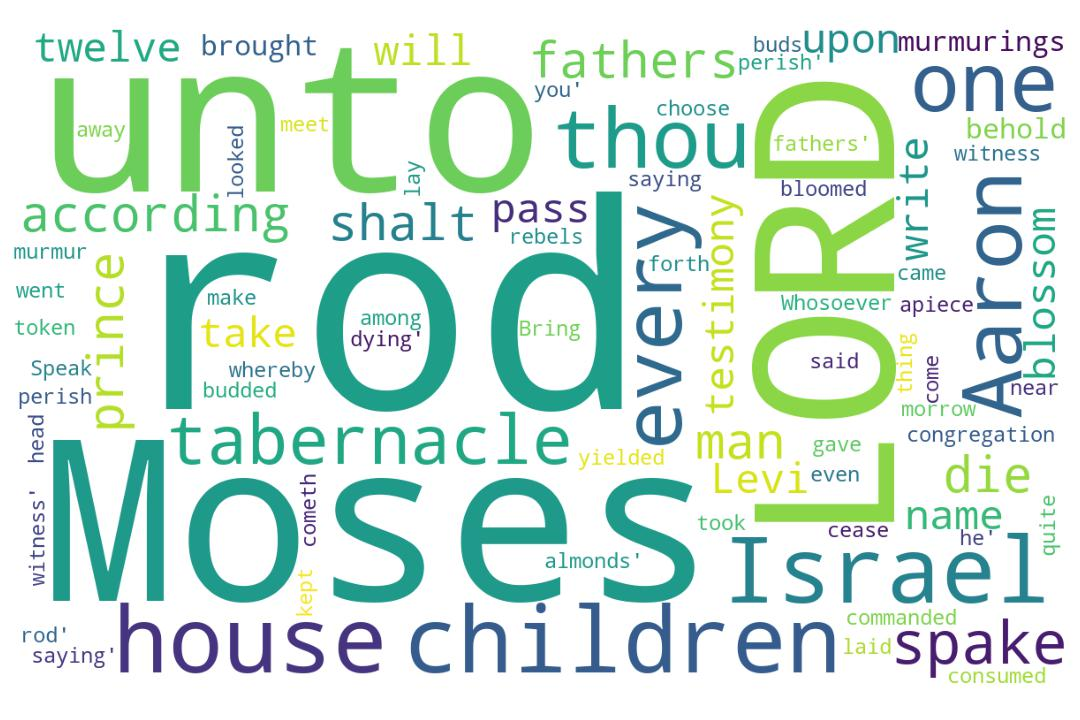
\includegraphics[width=\linewidth]{04OT-Numbers/Numbers17-WordCloud.jpg}
  \caption{Numbers 17 Word Cloud}
  \label{fig:Numbers 17 word Cloud}
\end{figure}

\marginpar{\scriptsize \centering \fcolorbox{bone}{lime}{\textbf{SHHHH}}\\ (Numbers 17:1-13) \begin{compactenum}[I.][8]
    \item  \textbf{Placement} \index[scripture]{Numbers!Num 17:04} (Numbers 17:4) 
    \item  \textbf{Purpose} \index[scripture]{Numbers!Num 17:05} (Numbers 17:5) 
    \item  \textbf{Princes} \index[scripture]{Numbers!Num 17:06} (Numbers 17:6) 
    \item  \textbf{Presence} \index[scripture]{Numbers!Num 17:07} (Numbers 17:7) 
    \item  \textbf{Prevention} \index[scripture]{Numbers!Num 17:10} (Numbers 17:10) 
    \item  \textbf{Perishing} \index[scripture]{Numbers!Num 17:12} (Numbers 17:12) 
    \item  \textbf{Pruning} %\index[scripture]{Numbers!Num 17:12} (Numbers 17:12) 
\end{compactenum}}
    



\footnote{\textcolor[cmyk]{0.99998,1,0,0}{\hyperlink{TOC}{Return to end of Table of Contents.}}}\footnote{\href{https://audiobible.com/bible/numbers_17.html}{\textcolor[cmyk]{0.99998,1,0,0}{Numbers 17 Audio}}}\textcolor[cmyk]{0.99998,1,0,0}{And the LORD spake unto Moses, saying,}
[2] \textcolor[cmyk]{0.99998,1,0,0}{Speak unto the children of Israel, and take of every one of them a rod according to the house of \emph{their} fathers, of all their princes according to the house of their fathers twelve rods: write thou every man's name upon his rod.}
[3] \textcolor[cmyk]{0.99998,1,0,0}{And thou shalt write Aaron's name upon the rod of Levi: for one rod \emph{shall} \emph{be} for the head of the house of their fathers.}
[4] \textcolor[cmyk]{0.99998,1,0,0}{And thou shalt lay them up \fcolorbox{bone}{lime}{in the tabernacle} of the congregation before the testimony, where I will meet with you.}
[5] \textcolor[cmyk]{0.99998,1,0,0}{And it shall come to pass, \emph{that} the man's rod, whom I shall choose, \fcolorbox{bone}{lime}{shall blossom}: and I will make to cease from me the murmurings of the children of Israel, whereby they murmur against you.}\\
\\
\P \textcolor[cmyk]{0.99998,1,0,0}{And Moses spake unto the children of Israel, and every one of their \fcolorbox{bone}{lime}{princes} gave him a rod apiece, for each prince one, according to their fathers' houses, \emph{even} twelve rods: and the rod of Aaron \emph{was} among their rods.}
[7] \textcolor[cmyk]{0.99998,1,0,0}{And Moses laid up the rods \fcolorbox{bone}{lime}{before the LORD} in the tabernacle of witness.}
[8] \textcolor[cmyk]{0.99998,1,0,0}{And it came to pass, that on the morrow Moses went into the tabernacle of witness; and, behold, the rod of Aaron for the house of Levi was budded, and brought forth buds, and bloomed blossoms, and yielded almonds.}\footnote{\textbf{Hebrews 9:4} - Which had the golden censer, and the ark of the covenant overlaid round about with gold, wherein was the golden pot that had manna, and Aaron’s rod that budded, and the tables of the covenant;}
[9] \textcolor[cmyk]{0.99998,1,0,0}{And Moses brought out all the rods from before the LORD unto all the children of Israel: and they looked, and took every man his rod.}\\
\\
\P \textcolor[cmyk]{0.99998,1,0,0}{And the LORD said unto Moses, Bring Aaron's rod again before the testimony, to be kept for a token \fcolorbox{bone}{lime}{against the rebels}; and thou shalt quite take away their murmurings from me, that they die not.}
[11] \textcolor[cmyk]{0.99998,1,0,0}{And Moses did \emph{so}: as the LORD commanded him, so did he.}
[12] \textcolor[cmyk]{0.99998,1,0,0}{And the children of Israel spake unto Moses, saying, Behold, we die, we \fcolorbox{bone}{lime}{perish}, we all perish.}
[13] \textcolor[cmyk]{0.99998,1,0,0}{Whosoever cometh any thing near unto the tabernacle of the LORD shall die: shall we be consumed with dying?}
\chapter{Numbers 18}

\begin{figure}
  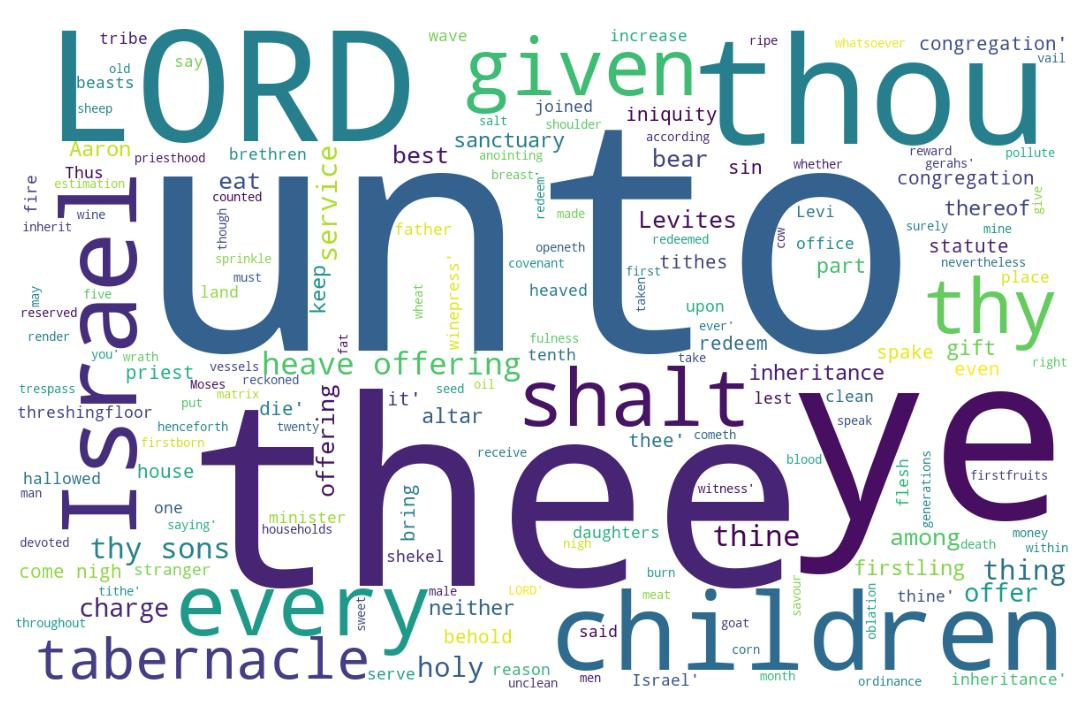
\includegraphics[width=\linewidth]{04OT-Numbers/Numbers18-WordCloud.jpg}
  \caption{Numbers 18 Word Cloud}
  \label{fig:Numbers 18 word Cloud}
\end{figure}


\marginpar{\scriptsize \centering \fcolorbox{bone}{lime}{\textbf{THE AARONIC PRIESTHOOD}}\\ (Numbers 18:1-32) \begin{compactenum}[I.][8]
    \item  \textbf{Sanctuary} \index[scripture]{Numbers!Num 18:01} \index[scripture]{Numbers!Num 18:03}\index[scripture]{Numbers!Num 18:05}\index[scripture]{Numbers!Num 18:16}(Numbers 18:1, 3, 5, 16) -- access to the sanctuary
    \item  \textbf{Sons} \index[scripture]{Numbers!Num 18:01} \index[scripture]{Numbers!Num 18:02}\index[scripture]{Numbers!Num 18:07}\index[scripture]{Numbers!Num 18:08}\index[scripture]{Numbers!Num 18:09}\index[scripture]{Numbers!Num 18:11}\index[scripture]{Numbers!Num 18:19} (Numbers 18:1, 2, 7, 8, 9, 11, 19) -- there is a family relationship between the priests. Here is the Aaronic priesthood. Elsewhere, see the priesthood of Melchisedek!
    \item  \textbf{Service} \index[scripture]{Numbers!Num 18:04} \index[scripture]{Numbers!Num 18:06}\index[scripture]{Numbers!Num 18:07}\index[scripture]{Numbers!Num 18:21}\index[scripture]{Numbers!Num 18:31}(Numbers 18:4, 6, 7, 21, 23, 31) -- the priests had duties of service
    \item  \textbf{Strangers} \index[scripture]{Numbers!Num 18:04} \index[scripture]{Numbers!Num 18:07}  (Numbers 18:4, 7) -- The strangers, people not part of God's fold, have no business with the priesthood
    \item  \textbf{Statutes} \index[scripture]{Numbers!Num 18:11} \index[scripture]{Numbers!Num 18:19}\index[scripture]{Numbers!Num 18:23} (Numbers 18:11, 19, 23) -- There are rules, God-given rules, for accessing and serving God
    \item  \textbf{Sin \& Sinners} \index[scripture]{Numbers!Num 18:09} \index[scripture]{Numbers!Num 18:22}\index[scripture]{Numbers!Num 18:26} \index[scripture]{Numbers!Num 18:32}(Numbers 18:9, 22, 26, 32) -- That sin problem -- always there to be dealt with
\end{compactenum}}
    




\footnote{\textcolor[cmyk]{0.99998,1,0,0}{\hyperlink{TOC}{Return to end of Table of Contents.}}}\footnote{\href{https://audiobible.com/bible/numbers_18.html}{\textcolor[cmyk]{0.99998,1,0,0}{Numbers 18 Audio}}}\textcolor[cmyk]{0.99998,1,0,0}{And the LORD said unto Aaron, Thou and thy \fcolorbox{bone}{lime}{sons} and thy father's house with thee shall bear the iniquity of the \fcolorbox{bone}{lime}{sanctuary}: and thou and thy sons with thee shall bear the iniquity of your priesthood.}
[2] \textcolor[cmyk]{0.99998,1,0,0}{And thy brethren also of the tribe of Levi, the tribe of thy father, bring thou with thee, that they may \fcolorbox{bone}{bone}{be} joined unto thee, and minister unto thee: but thou and thy \fcolorbox{bone}{lime}{sons} with thee \emph{shall} \emph{minister} before the tabernacle of witness.}
[3] \textcolor[cmyk]{0.99998,1,0,0}{And they shall keep thy charge, and the charge of all the tabernacle: only they shall not come nigh the vessels of the \fcolorbox{bone}{lime}{sanctuary} and the altar, that neither they, nor ye also, die.}
[4] \textcolor[cmyk]{0.99998,1,0,0}{And they shall \fcolorbox{bone}{bone}{be} joined unto thee, and keep the charge of the tabernacle of the congregation, for all the \fcolorbox{bone}{lime}{service} of the tabernacle: and \fcolorbox{bone}{bone}{a} \fcolorbox{bone}{lime}{stranger} shall not come nigh unto you.}
[5] \textcolor[cmyk]{0.99998,1,0,0}{And ye shall keep the charge of the \fcolorbox{bone}{lime}{sanctuary}, and the charge of the altar: that there \fcolorbox{bone}{bone}{be} no wrath any more upon \fcolorbox{bone}{bone}{the children of Israel}.}
[6] \textcolor[cmyk]{0.99998,1,0,0}{And \fcolorbox{bone}{bone}{I}, behold, \fcolorbox{bone}{bone}{I} have taken your brethren the Levites from among \fcolorbox{bone}{bone}{the children of Israel}: to you \emph{they} \emph{are} given \emph{as} \fcolorbox{bone}{bone}{a} gift for the LORD, to do the \fcolorbox{bone}{lime}{service} of the tabernacle of the congregation.}
[7] \textcolor[cmyk]{0.99998,1,0,0}{Therefore thou and thy \fcolorbox{bone}{lime}{sons} with thee shall keep your priest's office for every thing of the altar, and within the vail; and ye shall serve: \fcolorbox{bone}{bone}{I} have given your priest's office \emph{unto} \emph{you} as \fcolorbox{bone}{bone}{a} \fcolorbox{bone}{lime}{service} of gift: and the \fcolorbox{bone}{lime}{stranger} that cometh nigh shall \fcolorbox{bone}{bone}{be} put to death.}\\
\\
\P \textcolor[cmyk]{0.99998,1,0,0}{And the LORD spake unto Aaron, Behold, \fcolorbox{bone}{bone}{I} also have given thee the charge of mine heave offerings of all the hallowed things of \fcolorbox{bone}{bone}{the children of Israel}; unto thee have \fcolorbox{bone}{bone}{I} given them by reason of the anointing, and to thy \fcolorbox{bone}{lime}{sons}, by an ordinance for ever.}
[9] \textcolor[cmyk]{0.99998,1,0,0}{This shall \fcolorbox{bone}{bone}{be} thine of the most holy things, \emph{reserved} from the fire: every oblation of their's, every meat offering of their's, and every \fcolorbox{bone}{lime}{sin} offering of their's, and every trespass offering of their's, which they shall render unto me, \emph{shall} \emph{be} most holy for thee and for thy \fcolorbox{bone}{lime}{sons}.}
[10] \textcolor[cmyk]{0.99998,1,0,0}{In the most holy \emph{place} shalt thou eat it; every male shall eat it: it shall \fcolorbox{bone}{bone}{be} holy unto thee.}
[11] \textcolor[cmyk]{0.99998,1,0,0}{And this \emph{is} thine; the heave offering of their gift, with all the wave offerings of \fcolorbox{bone}{bone}{the children of Israel}: \fcolorbox{bone}{bone}{I} have given them unto thee, and to thy \fcolorbox{bone}{lime}{sons} and to thy daughters with thee, by \fcolorbox{bone}{bone}{a} \fcolorbox{bone}{lime}{statute} for ever: every one that is clean in thy house shall eat of it.}
[12] \textcolor[cmyk]{0.99998,1,0,0}{All the best of the oil, and all the best of the wine, and of the wheat, the firstfruits of them which they shall offer unto the LORD, them have \fcolorbox{bone}{bone}{I} given thee.}
[13] \textcolor[cmyk]{0.99998,1,0,0}{\emph{And} whatsoever is first ripe in the land, which they shall bring unto the LORD, shall \fcolorbox{bone}{bone}{be} thine; every one that is clean in thine house shall eat \emph{of} it.}
[14] \textcolor[cmyk]{0.99998,1,0,0}{Every thing devoted in Israel shall \fcolorbox{bone}{bone}{be} thine.}
[15] \textcolor[cmyk]{0.99998,1,0,0}{Every thing that openeth the matrix in all flesh, which they bring unto the LORD, \emph{whether} \emph{it} \emph{be} of men or beasts, shall \fcolorbox{bone}{bone}{be} thine: nevertheless the firstborn of man shalt thou surely redeem, and the firstling of unclean beasts shalt thou redeem.}
[16] \textcolor[cmyk]{0.99998,1,0,0}{And those that are to \fcolorbox{bone}{bone}{be} redeemed from \fcolorbox{bone}{bone}{a} month old shalt thou redeem, according to thine estimation, for the money of five shekels, after the shekel of the \fcolorbox{bone}{lime}{sanctuary}, which \emph{is} twenty gerahs.}
[17] \textcolor[cmyk]{0.99998,1,0,0}{But the firstling of \fcolorbox{bone}{bone}{a} cow, or the firstling of \fcolorbox{bone}{bone}{a} sheep, or the firstling of \fcolorbox{bone}{bone}{a} goat, thou shalt not redeem; they \emph{are} holy: thou shalt sprinkle their blood upon the altar, and shalt burn their fat \emph{for} an offering made by fire, for \fcolorbox{bone}{bone}{a} sweet savour unto the LORD.}
[18] \textcolor[cmyk]{0.99998,1,0,0}{And the flesh of them shall \fcolorbox{bone}{bone}{be} thine, as the wave breast and as the right shoulder are thine.}
[19] \textcolor[cmyk]{0.99998,1,0,0}{All the heave offerings of the holy things, which \fcolorbox{bone}{bone}{the children of Israel} offer unto the LORD, have \fcolorbox{bone}{bone}{I} given thee, and thy \fcolorbox{bone}{lime}{sons} and thy daughters with thee, by \fcolorbox{bone}{bone}{a} \fcolorbox{bone}{lime}{statute} for ever: it \emph{is} \fcolorbox{bone}{bone}{a} covenant of salt for ever before the LORD unto thee and to thy seed with thee.}\\
\\
\P \textcolor[cmyk]{0.99998,1,0,0}{And the LORD spake unto Aaron, Thou shalt have no inheritance in their land, neither shalt thou have any part among them: \fcolorbox{bone}{bone}{I} \emph{am} thy part and thine inheritance among \fcolorbox{bone}{bone}{the children of Israel}.}
[21] \textcolor[cmyk]{0.99998,1,0,0}{And, behold, \fcolorbox{bone}{bone}{I} have given the children of Levi all the tenth in Israel for an inheritance, for their service which they serve, \emph{even} the \fcolorbox{bone}{lime}{service} of the tabernacle of the congregation.}
[22] \textcolor[cmyk]{0.99998,1,0,0}{Neither must \fcolorbox{bone}{bone}{the children of Israel} henceforth come nigh the tabernacle of the congregation, lest they bear \fcolorbox{bone}{lime}{sin}, and die.}
[23] \textcolor[cmyk]{0.99998,1,0,0}{But the Levites shall do the \fcolorbox{bone}{lime}{service} of the tabernacle of the congregation, and they shall bear their iniquity: \emph{it} \emph{shall} \emph{be} \fcolorbox{bone}{bone}{a} \fcolorbox{bone}{lime}{statute} for ever throughout your generations, that among \fcolorbox{bone}{bone}{the children of Israel} they have no inheritance.}
[24] \textcolor[cmyk]{0.99998,1,0,0}{But the tithes of \fcolorbox{bone}{bone}{the children of Israel}, which they offer \emph{as} an heave offering unto the LORD, \fcolorbox{bone}{bone}{I} have given to the Levites to inherit: therefore \fcolorbox{bone}{bone}{I} have said unto them, Among \fcolorbox{bone}{bone}{the children of Israel} they shall have no inheritance.}\\
\\
\P \textcolor[cmyk]{0.99998,1,0,0}{And the LORD spake unto Moses, saying,}
[26] \textcolor[cmyk]{0.99998,1,0,0}{Thus speak unto the Levites, and say unto them, When ye take of \fcolorbox{bone}{bone}{the children of Israel} the tithes which \fcolorbox{bone}{bone}{I} have given you from them for your inheritance, then ye shall offer up an heave offering of it for the LORD, \emph{even} \fcolorbox{bone}{bone}{a} tenth \emph{part} of the tithe.}
[27] \textcolor[cmyk]{0.99998,1,0,0}{And \emph{this} your heave offering shall \fcolorbox{bone}{bone}{be} reckoned unto you, as though \emph{it} \emph{were} the corn of the threshingfloor, and as the fulness of the winepress.}
[28] \textcolor[cmyk]{0.99998,1,0,0}{Thus ye also shall offer an heave offering unto the LORD of all your tithes, which ye receive of \fcolorbox{bone}{bone}{the children of Israel}; and ye shall give thereof the LORD'S heave offering to Aaron the priest.}
[29] \textcolor[cmyk]{0.99998,1,0,0}{Out of all your gifts ye shall offer every heave offering of the LORD, of all the best thereof, \emph{even} the hallowed part thereof out of it.}
[30] \textcolor[cmyk]{0.99998,1,0,0}{Therefore thou shalt say unto them, When ye have heaved the best thereof from it, then it shall \fcolorbox{bone}{bone}{be} counted unto the Levites as the increase of the threshingfloor, and as the increase of the winepress.}
[31] \textcolor[cmyk]{0.99998,1,0,0}{And ye shall eat it in every place, ye and your households: for it \emph{is} your reward for your \fcolorbox{bone}{lime}{service} in the tabernacle of the congregation.}
[32] \textcolor[cmyk]{0.99998,1,0,0}{And ye shall bear no \fcolorbox{bone}{lime}{sin} by reason of it, when ye have heaved from it the best of it: neither shall ye pollute the holy things of \fcolorbox{bone}{bone}{the children of Israel}, lest ye die.}

\chapter{Psalm 46}

\begin{figure}
  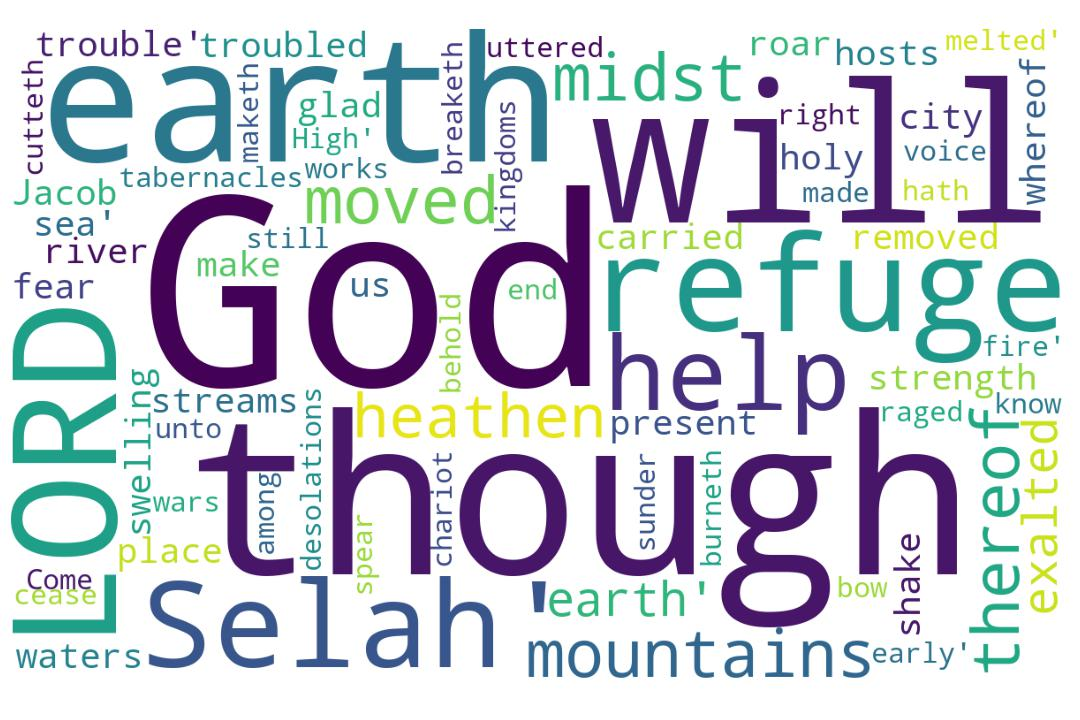
\includegraphics[width=\linewidth]{19OT-Psalms/Psalm46-WordCloud.jpg}
  \caption{Psalm 46 Word Cloud}
  \label{fig:Psalm 46 word Cloud}
\end{figure}

\marginpar{\scriptsize \centering \fcolorbox{bone}{lime}{\textbf{THERE IS A REFUGE}}\\ (Psalm 46) 
\begin{compactenum}[I.][8]
	\item There is a \textbf{Refuge} \index[scripture]{Psalms!Psa 046:01}\index[scripture]{Psalms!Psa 046:07}\index[scripture]{Psalms!Psa 046:11}(Psalm 46:1, 7, 11)
	\item There is a \textbf{Removal} of Evil \index[scripture]{Psalms!Psa 046:02}(Psa 46:2)
	\item There is a \textbf{River} of Life -- for God's People \index[scripture]{Psalms!Psa 046:04}(Psa 46:4)
	\item There is a \textbf{Raging} by God's Enemies \index[scripture]{Psalms!Psa 046:06}(Psa 46:6)
	\item There is \textbf{Ruin} for Evil \index[scripture]{Psalms!Psa 046:08}(Psa 46:8)
	\item There is a \textbf{Resolution} of the Conflict between Good and Evil \index[scripture]{Psalms!Psa 046:09}(Psa 46:9)
	\item There is a \textbf{Remedy} for Sin \index[scripture]{Psalms!Psa 046:10}(Psa 46:10)
	\item There is a \textbf{Repose} for Righteousness \index[scripture]{Psalms!Psa 046:11}(Psa 46:11)
\end{compactenum}}
    
\marginpar{\scriptsize \centering \fcolorbox{bone}{yellow}{\textbf{THERE IS A REFUGE}}\\ (Psalm 46) 
\begin{compactenum}[I.][8]
    \item \textbf{Welcome} of the Lord \index[scripture]{Psalms!Psa 046:01}\index[scripture]{Psalms!Psa 046:11} (Psa 46:1, 11)
    \item The \textbf{Water} of the Lord \index[scripture]{Psalms!Psa 046:04} (Psa 46:4)
    \item The \textbf{Words} of the Lord \index[scripture]{Psalms!Psa 046:06} (Psa 46:6)
    \item The \textbf{Works} of the Lord \index[scripture]{Psalms!Psa 046:08} (Psa 46:8)
    \item The \textbf{Wrath} of the Lord \index[scripture]{Psalms!Psa 046:09} (Psa 46:9)
    \item The \textbf{Wars} of the Lord \index[scripture]{Psalms!Psa 046:09} (Psa 46:9)
    \item The \textbf{Worship} of the Lord \index[scripture]{Psalms!Psa 046:10} (Psa 46:10)
\end{compactenum}}

\footnote{\textcolor[cmyk]{0.99998,1,0,0}{\hyperlink{TOC}{Return to end of Table of Contents.}}}\footnote{\href{https://audiobible.com/bible/psalms_46.html}{\textcolor[cmyk]{0.99998,1,0,0}{Psalms Audio}}}\textcolor[cmyk]{0.99998,1,0,0}{To the chief Musician for the sons of Korah, A Song upon Alamoth.}\\
\\
\textcolor[cmyk]{0.99998,1,0,0}{God \emph{is} our \fcolorbox{bone}{lime}{refuge} and strength, a very present help in trouble.}
[2] \textcolor[cmyk]{0.99998,1,0,0}{Therefore will not we fear, though the earth be \fcolorbox{bone}{lime}{removed}, and though the mountains be carried into the midst of the sea;}
[3] \textcolor[cmyk]{0.99998,1,0,0}{\emph{Though} the waters thereof roar \emph{and} be troubled, \emph{though} the mountains shake with the swelling thereof. Selah.}
[4] \textcolor[cmyk]{0.99998,1,0,0}{\emph{There} \emph{is} a \fcolorbox{bone}{lime}{river}, the streams whereof shall make glad the city of God, the holy \emph{place} of the tabernacles of the most High.}
[5] \textcolor[cmyk]{0.99998,1,0,0}{God \emph{is} in the midst of her; she shall not be moved: God shall help her, \emph{and} \emph{that} right early.}
[6] \textcolor[cmyk]{0.99998,1,0,0}{The heathen \fcolorbox{bone}{lime}{raged}, the kingdoms were moved: he uttered his voice, the earth melted.}\footnote{\textbf{Psalm 2:1} - Why do the heathen rage, and the people imagine a vain thing?, with \textbf{Acts 4:25} - Who by the mouth of thy servant David hast said, Why did the heathen rage, and the people imagine vain things?}\footnote{\textbf{Judges 5:5} - The mountains melted from before the LORD, even that Sinai from before the LORD God of Israel.}\footnote{\textbf{Psalm 97:5} - The hills melted like wax at the presence of the LORD, at the presence of the Lord of the whole earth.}\footnote{\textbf{Amos 9:5} - And the Lord GOD of hosts is he that toucheth the land, and it shall melt, and all that dwell therein shall mourn: and it shall rise up wholly like a flood; and shall be drowned, as by the flood of Egypt.}\footnote{\textbf{Amos 9:13} - Behold, the days come, saith the LORD, that the plowman shall overtake the reaper, and the treader of grapes him that soweth seed; and the mountains shall drop sweet wine, and all the hills shall melt.}\footnote{\textbf{Nahum 1:5} - The mountains quake at him, and the hills melt, and the earth is burned at his presence, yea, the world, and all that dwell therein.}\footnote{\textbf{2 Peter 3:10-12} - But the day of the Lord will come as a thief in the night; in the which the heavens shall pass away with a great noise, and the elements shall melt with fervent heat, the earth also and the works that are therein shall be burned up. [11] Seeing then that all these things shall be dissolved, what manner of persons ought ye to be in all holy conversation and godliness, [12] Looking for and hasting unto the coming of the day of God, wherein the heavens being on fire shall be dissolved, and the elements shall melt with fervent heat?}
[7] \textcolor[cmyk]{0.99998,1,0,0}{The LORD of hosts \emph{is} with us; the God of Jacob \emph{is} our \fcolorbox{bone}{lime}{refuge}. Selah.}
[8] \textcolor[cmyk]{0.99998,1,0,0}{Come, behold the works of the LORD, what \fcolorbox{bone}{lime}{desolations} he hath made in the earth.}\footnote{\textbf{Psalm 73:19} - How are they brought into desolation, as in a moment! they are utterly consumed with terrors.}\footnote{\textbf{Isaiah 10:3} - And what will ye do in the day of visitation, and in the desolation which shall come from far? to whom will ye flee for help? and where will ye leave your glory?}\footnote{\textbf{Isaiah 61:4} - And they shall build the old wastes, they shall raise up the former desolations, and they shall repair the waste cities, the desolations of many generations.}
[9] \textcolor[cmyk]{0.99998,1,0,0}{He maketh wars to cease unto the end of the earth; he breaketh the bow, and cutteth the spear in sunder; he burneth the chariot in the fire.}\marginpar{\scriptsize \textcolor[rgb]{0.00,0.545,0.269}{Four things the Lord does:
\begin{compactenum}
\item Maketh wars to cease
\item Breaketh the bow
\item Cutteth the spear in sunder
\item Burneth the chariot in the fire
\end{compactenum}} }\footnote{\textbf{Isaiah 2:4} - And he shall judge among the nations, and shall rebuke many people: and they shall beat their swords into plowshares, and their spears into pruninghooks: nation shall not lift up sword against nation, neither shall they learn war any more.}\footnote{\textbf{Joel 3:10} - Beat your plowshares into swords, and your pruninghooks into spears: let the weak say, I am strong.}\footnote{\textbf{Micah 4:3-7} - And he shall judge among many people, and rebuke strong nations afar off; and they shall beat their swords into plowshares, and their spears into pruninghooks: nation shall not lift up a sword against nation, neither shall they learn war any more. [4] But they shall sit every man under his vine and under his fig tree; and none shall make them afraid: for the mouth of the LORD of hosts hath spoken it. [5] For all people will walk every one in the name of his god, and we will walk in the name of the LORD our God for ever and ever. [6] In that day, saith the LORD, will I assemble her that halteth, and I will gather her that is driven out, and her that I have afflicted; [7] And I will make her that halted a remnant, and her that was cast far off a strong nation: and the LORD shall reign over them in mount Zion from henceforth, even for ever.}
[10] \textcolor[cmyk]{0.99998,1,0,0}{Be still, and know that I \emph{am} God: I will be \fcolorbox{bone}{lime}{exalted} among the heathen, I will be exalted in the earth.}
[11] \textcolor[cmyk]{0.99998,1,0,0}{The LORD of hosts \emph{is} with us; the God of Jacob \emph{is} our \fcolorbox{bone}{lime}{refuge}. Selah.}





\chapter{Proverb 15}\marginpar{\scriptsize \centering \fcolorbox{bone}{lime}{\textbf{RIGHTEOUS LIPS}}\\ (Proverbs 15:1-33) \begin{compactenum}[I.][8]
    \item \textbf{Turn Away Wrath}  \index[scripture]{Proverbs!Pro 15:01}(Pro 15:1)
    \item \textbf{Dispense Knowledge} \index[scripture]{Proverbs!Pro 15:02, 07}(Pro 15:2, 7)
    \item \textbf{Are Wholesome} \index[scripture]{Proverbs!Pro 15:04}(Pro 15:4)
    \item \textbf{Offer counsel} \index[scripture]{Proverbs!Pro 15:22}(Pro 15:22)
    \item \textbf{Speak in Due Season} \index[scripture]{Proverbs!Pro 15:23}(Pro 15:23)
    \item \textbf{Are Pure and Pleasant} \index[scripture]{Proverbs!Pro 15:26}(Pro 15:26)
    \item \textbf{Answer Slowly} \index[scripture]{Proverbs!Pro 15:28}(Pro 15:28) -- some answers are not easy
\end{compactenum}}

\marginpar{\scriptsize \centering \fcolorbox{bone}{yellow}{\textbf{RESPONDING TO CORRECTION}}\\ (Proverbs 15:1-33) \begin{compactenum}[I.][8]
    \item \textbf{Wrath}  \index[scripture]{Proverbs!Pro 15:01} 
                                      \index[scripture]{Proverbs!Pro 15:18} 
                                      (Pro 15:1, 18)
    \item \textbf{Reproof}  \index[scripture]{Proverbs!Pro 15:05} 
                                      \index[scripture]{Proverbs!Pro 15:10} 
                                      \index[scripture]{Proverbs!Pro 15:12} 
                                      \index[scripture]{Proverbs!Pro 15:31} 
                                      \index[scripture]{Proverbs!Pro 15:32}  (Pro 15:5, 10, 12, 31, 32)
    \item God's \textbf{Reconnaissance}  \index[scripture]{Proverbs!Pro 15:03}  (Pro 15:3)
    \item \textbf{Regard}  \index[scripture]{Proverbs!Pro 15:05}  (Pro 15:5)
    \item \textbf{Righteousness}  \index[scripture]{Proverbs!Pro 15:06} \index[scripture]{Proverbs!Pro 15:09} \index[scripture]{Proverbs!Pro 15:19} \index[scripture]{Proverbs!Pro 15:28} 
    \index[scripture]{Proverbs!Pro 15:29}  (Pro 15:6, 9, 19, 28, 29)
    \item \textbf{Refusal}  \index[scripture]{Proverbs!Pro 15:32}  (Pro 15:32)
    \item \textbf{Receiving}  \index[scripture]{Proverbs!Pro 15:32}  (Pro 15:32)
\end{compactenum}}
    
\footnote{\textcolor[cmyk]{0.99998,1,0,0}{\hyperlink{TOC}{Return to end of Table of Contents.}}}\footnote{\href{https://audiobible.com/bible/proverbs_15.html}{\textcolor[cmyk]{0.99998,1,0,0}{Proverbs Audio}}}\textcolor[cmyk]{0.99998,1,0,0}{A soft answer \fcolorbox{bone}{lime}{turneth away wrath}: but grievous words stir up anger.}
[2] \textcolor[cmyk]{0.99998,1,0,0}{The tongue of the wise \fcolorbox{bone}{lime}{useth knowledge} aright: but the mouth of fools poureth out foolishness.}
[3] \textcolor[cmyk]{0.99998,1,0,0}{The eyes of the LORD \emph{are} in every place, beholding the evil and the good.}
[4] \textcolor[cmyk]{0.99998,1,0,0}{\fcolorbox{bone}{lime}{A wholesome tongue} \emph{is} a tree of life: but perverseness therein \emph{is} a breach in the spirit.}
[5] \textcolor[cmyk]{0.99998,1,0,0}{A fool despiseth his father's instruction: but he \fcolorbox{bone}{bone}{that} regardeth reproof is prudent.}
[6] \textcolor[cmyk]{0.99998,1,0,0}{In the house of the righteous \emph{is} much treasure: but in the revenues of the wicked is trouble.}
[7] \textcolor[cmyk]{0.99998,1,0,0}{The lips of the wise \fcolorbox{bone}{lime}{disperse knowledge}: but the heart of the foolish \emph{doeth} not so.}
[8] \textcolor[cmyk]{0.99998,1,0,0}{The sacrifice of the wicked \emph{is} an abomination to the LORD: but the prayer of the upright \emph{is} his delight.}
[9] \textcolor[cmyk]{0.99998,1,0,0}{The way of the wicked \emph{is} an abomination unto the LORD: but he loveth him \fcolorbox{bone}{bone}{that} followeth after righteousness.}
[10] \textcolor[cmyk]{0.99998,1,0,0}{Correction \emph{is} grievous unto him \fcolorbox{bone}{bone}{that} forsaketh the way: \emph{and} he \fcolorbox{bone}{bone}{that} hateth reproof shall die.}\footnote{\textbf{Jeremiah 2:30} - In vain have I smitten your children; they received no correction: your own sword hath devoured your prophets, like a destroying lion.}\footnote{\textbf{Jeremiah 5:3} - O LORD, are not thine eyes upon the truth? thou hast stricken them, but they have not grieved; thou hast consumed them, but they have refused to receive correction: they have made their faces harder than a rock; they have refused to return.}\footnote{\textbf{Jeremiah 7:28} - But thou shalt say unto them, This is a nation that obeyeth not the voice of the LORD their God, nor receiveth correction: truth is perished, and is cut off from their mouth.}\footnote{\textbf{Zephaniah 3:2} - She obeyed not the voice; she received not correction; she trusted not in the LORD; she drew not near to her God.}\footnote{\textbf{2 Timothy 3:16} - All scripture is given by inspiration of God, and is profitable for doctrine, for reproof, for correction, for instruction in righteousness:}
[11] \textcolor[cmyk]{0.99998,1,0,0}{Hell and destruction \emph{are} before the LORD: how much more then the hearts of the children of men?}
[12] \textcolor[cmyk]{0.99998,1,0,0}{A scorner loveth not one \fcolorbox{bone}{bone}{that} reproveth him: neither will he go unto the wise.}
[13] \textcolor[cmyk]{0.99998,1,0,0}{A merry heart maketh a cheerful countenance: but by sorrow of the heart the spirit is broken.}
[14] \textcolor[cmyk]{0.99998,1,0,0}{The heart of him \fcolorbox{bone}{bone}{that} hath understanding seeketh knowledge: but the mouth of fools feedeth on foolishness.}
[15] \textcolor[cmyk]{0.99998,1,0,0}{All the days of the afflicted \emph{are} evil: but he \fcolorbox{bone}{bone}{that} is of a merry heart \emph{hath} a continual feast.}
[16] \textcolor[cmyk]{0.99998,1,0,0}{Better \emph{is} little with the fear of the LORD than great treasure and trouble therewith.}
[17] \textcolor[cmyk]{0.99998,1,0,0}{Better \emph{is} a dinner of herbs where love is, than a stalled ox and hatred therewith.}
[18] \textcolor[cmyk]{0.99998,1,0,0}{A wrathful man stirreth up strife: but \emph{he} \emph{that} \emph{is} slow to anger appeaseth strife.}
[19] \textcolor[cmyk]{0.99998,1,0,0}{The way of the slothful \emph{man} \emph{is} as an hedge of thorns: but the way of the righteous \emph{is} made plain.}
[20] \textcolor[cmyk]{0.99998,1,0,0}{A wise son maketh a glad father: but a foolish man despiseth his mother.}
[21] \textcolor[cmyk]{0.99998,1,0,0}{Folly \emph{is} joy to \emph{him} \emph{that} \emph{is} destitute of wisdom: but a man of understanding walketh uprightly.}
[22] \textcolor[cmyk]{0.99998,1,0,0}{Without \fcolorbox{bone}{lime}{counsel} purposes are disappointed: but in the multitude of \fcolorbox{bone}{lime}{counsellors} they are established.}
[23] \textcolor[cmyk]{0.99998,1,0,0}{A man hath joy by the answer of his mouth: and a word \emph{spoken} \fcolorbox{bone}{lime}{in due season}, how good \emph{is} \emph{it}!}
[24] \textcolor[cmyk]{0.99998,1,0,0}{The way of life \emph{is} above to the wise, \fcolorbox{bone}{bone}{that} he may depart from hell beneath.}
[25] \textcolor[cmyk]{0.99998,1,0,0}{The LORD will destroy the house of the proud: but he will establish the border of the widow.}
[26] \textcolor[cmyk]{0.99998,1,0,0}{The thoughts of the wicked \emph{are} an abomination to the LORD: but \emph{the} \emph{words} of the pure \emph{are} \fcolorbox{bone}{lime}{pleasant words}.}
[27] \textcolor[cmyk]{0.99998,1,0,0}{He \fcolorbox{bone}{bone}{that} is greedy of gain troubleth his own house; but he \fcolorbox{bone}{bone}{that} hateth gifts shall live.}
[28] \textcolor[cmyk]{0.99998,1,0,0}{The heart of the righteous \fcolorbox{bone}{lime}{studieth to answer}: but the mouth of the wicked poureth out evil things.}
[29] \textcolor[cmyk]{0.99998,1,0,0}{The LORD \emph{is} far from the wicked: but he heareth the prayer of the righteous.}
[30] \textcolor[cmyk]{0.99998,1,0,0}{The light of the eyes rejoiceth the heart: \emph{and} a good report maketh the bones fat.}
[31] \textcolor[cmyk]{0.99998,1,0,0}{The ear \fcolorbox{bone}{bone}{that} heareth the reproof of life abideth among the wise.}
[32] \textcolor[cmyk]{0.99998,1,0,0}{He \fcolorbox{bone}{bone}{that} refuseth instruction despiseth his own soul: but he \fcolorbox{bone}{bone}{that} heareth reproof getteth understanding.}
[33] \textcolor[cmyk]{0.99998,1,0,0}{The fear of the LORD \emph{is} the instruction of wisdom; and before honour \emph{is} humility.}




\end{document}

